\documentclass[twoside]{book}

% Packages required by doxygen
\usepackage{fixltx2e}
\usepackage{calc}
\usepackage{doxygen}
\usepackage[export]{adjustbox} % also loads graphicx
\usepackage{graphicx}
\usepackage[utf8]{inputenc}
\usepackage{makeidx}
\usepackage{multicol}
\usepackage{multirow}
\PassOptionsToPackage{warn}{textcomp}
\usepackage{textcomp}
\usepackage[nointegrals]{wasysym}
\usepackage[table]{xcolor}

% Font selection
\usepackage[T1]{fontenc}
\usepackage[scaled=.90]{helvet}
\usepackage{courier}
\usepackage{amssymb}
\usepackage{sectsty}
\renewcommand{\familydefault}{\sfdefault}
\allsectionsfont{%
  \fontseries{bc}\selectfont%
  \color{darkgray}%
}
\renewcommand{\DoxyLabelFont}{%
  \fontseries{bc}\selectfont%
  \color{darkgray}%
}
\newcommand{\+}{\discretionary{\mbox{\scriptsize$\hookleftarrow$}}{}{}}

% Page & text layout
\usepackage{geometry}
\geometry{%
  a4paper,%
  top=2.5cm,%
  bottom=2.5cm,%
  left=2.5cm,%
  right=2.5cm%
}
\tolerance=750
\hfuzz=15pt
\hbadness=750
\setlength{\emergencystretch}{15pt}
\setlength{\parindent}{0cm}
\setlength{\parskip}{3ex plus 2ex minus 2ex}
\makeatletter
\renewcommand{\paragraph}{%
  \@startsection{paragraph}{4}{0ex}{-1.0ex}{1.0ex}{%
    \normalfont\normalsize\bfseries\SS@parafont%
  }%
}
\renewcommand{\subparagraph}{%
  \@startsection{subparagraph}{5}{0ex}{-1.0ex}{1.0ex}{%
    \normalfont\normalsize\bfseries\SS@subparafont%
  }%
}
\makeatother

% Headers & footers
\usepackage{fancyhdr}
\pagestyle{fancyplain}
\fancyhead[LE]{\fancyplain{}{\bfseries\thepage}}
\fancyhead[CE]{\fancyplain{}{}}
\fancyhead[RE]{\fancyplain{}{\bfseries\leftmark}}
\fancyhead[LO]{\fancyplain{}{\bfseries\rightmark}}
\fancyhead[CO]{\fancyplain{}{}}
\fancyhead[RO]{\fancyplain{}{\bfseries\thepage}}
\fancyfoot[LE]{\fancyplain{}{}}
\fancyfoot[CE]{\fancyplain{}{}}
\fancyfoot[RE]{\fancyplain{}{\bfseries\scriptsize Generated by Doxygen }}
\fancyfoot[LO]{\fancyplain{}{\bfseries\scriptsize Generated by Doxygen }}
\fancyfoot[CO]{\fancyplain{}{}}
\fancyfoot[RO]{\fancyplain{}{}}
\renewcommand{\footrulewidth}{0.4pt}
\renewcommand{\chaptermark}[1]{%
  \markboth{#1}{}%
}
\renewcommand{\sectionmark}[1]{%
  \markright{\thesection\ #1}%
}

% Indices & bibliography
\usepackage{natbib}
\usepackage[titles]{tocloft}
\setcounter{tocdepth}{3}
\setcounter{secnumdepth}{5}
\makeindex

% Hyperlinks (required, but should be loaded last)
\usepackage{ifpdf}
\ifpdf
  \usepackage[pdftex,pagebackref=true]{hyperref}
\else
  \usepackage[ps2pdf,pagebackref=true]{hyperref}
\fi
\hypersetup{%
  colorlinks=true,%
  linkcolor=blue,%
  citecolor=blue,%
  unicode%
}

% Custom commands
\newcommand{\clearemptydoublepage}{%
  \newpage{\pagestyle{empty}\cleardoublepage}%
}

\usepackage{caption}
\captionsetup{labelsep=space,justification=centering,font={bf},singlelinecheck=off,skip=4pt,position=top}

%===== C O N T E N T S =====

\begin{document}

% Titlepage & ToC
\hypersetup{pageanchor=false,
             bookmarksnumbered=true,
             pdfencoding=unicode
            }
\pagenumbering{alph}
\begin{titlepage}
\vspace*{7cm}
\begin{center}%
{\Large Editor }\\
\vspace*{1cm}
{\large Generated by Doxygen 1.8.14}\\
\end{center}
\end{titlepage}
\clearemptydoublepage
\pagenumbering{roman}
\tableofcontents
\clearemptydoublepage
\pagenumbering{arabic}
\hypersetup{pageanchor=true}

%--- Begin generated contents ---
\chapter{Hierarchical Index}
\section{Class Hierarchy}
This inheritance list is sorted roughly, but not completely, alphabetically\+:\begin{DoxyCompactList}
\item \contentsline{section}{Bezier}{\pageref{classBezier}}{}
\item \contentsline{section}{Bezier\+\_\+\+Mode}{\pageref{structBezier__Mode}}{}
\item \contentsline{section}{Bezier\+Toolbar}{\pageref{structBezierToolbar}}{}
\item \contentsline{section}{End\+\_\+\+Points}{\pageref{structEnd__Points}}{}
\item \contentsline{section}{Image\+\_\+\+Active}{\pageref{structImage__Active}}{}
\item \contentsline{section}{Image\+\_\+\+Cut}{\pageref{structImage__Cut}}{}
\item \contentsline{section}{Line\+\_\+\+Mode}{\pageref{structLine__Mode}}{}
\item \contentsline{section}{Mode\+Toolbar}{\pageref{structModeToolbar}}{}
\item \contentsline{section}{Polygon\+Toolbar}{\pageref{structPolygonToolbar}}{}
\item Q\+Dialog\begin{DoxyCompactList}
\item \contentsline{section}{Promt\+Window}{\pageref{classPromtWindow}}{}
\end{DoxyCompactList}
\item Q\+Graphics\+Line\+Item\begin{DoxyCompactList}
\item \contentsline{section}{Line\+Item}{\pageref{classLineItem}}{}
\end{DoxyCompactList}
\item Q\+Graphics\+Pixmap\+Item\begin{DoxyCompactList}
\item \contentsline{section}{Pixmap\+Item}{\pageref{classPixmapItem}}{}
\end{DoxyCompactList}
\item Q\+Graphics\+Scene\begin{DoxyCompactList}
\item \contentsline{section}{Own\+Graphics\+Scene}{\pageref{classOwnGraphicsScene}}{}
\end{DoxyCompactList}
\item Q\+Graphics\+Text\+Item\begin{DoxyCompactList}
\item \contentsline{section}{Text\+Item}{\pageref{classTextItem}}{}
\end{DoxyCompactList}
\item Q\+Graphics\+View\begin{DoxyCompactList}
\item \contentsline{section}{Own\+Graphics\+View}{\pageref{classOwnGraphicsView}}{}
\end{DoxyCompactList}
\item Q\+Main\+Window\begin{DoxyCompactList}
\item \contentsline{section}{G\+UI}{\pageref{classGUI}}{}
\end{DoxyCompactList}
\item Q\+Widget\begin{DoxyCompactList}
\item \contentsline{section}{Main\+Widget}{\pageref{classMainWidget}}{}
\end{DoxyCompactList}
\item Q\+Widget\+Action\begin{DoxyCompactList}
\item \contentsline{section}{Combobox\+Action}{\pageref{classComboboxAction}}{}
\item \contentsline{section}{Spin\+Box\+Action}{\pageref{classSpinBoxAction}}{}
\end{DoxyCompactList}
\item \contentsline{section}{Select\+Img\+Toolbar}{\pageref{structSelectImgToolbar}}{}
\item \contentsline{section}{Vector2}{\pageref{classVector2}}{}
\item \contentsline{section}{X\+\_\+\+Y\+\_\+\+Coordinates}{\pageref{structX__Y__Coordinates}}{}
\end{DoxyCompactList}

\chapter{Class Index}
\section{Class List}
Here are the classes, structs, unions and interfaces with brief descriptions\+:\begin{DoxyCompactList}
\item\contentsline{section}{\mbox{\hyperlink{classComboboxAction}{Combobox\+Action}} \\*Implements own Q\+Combo\+Box }{\pageref{classComboboxAction}}{}
\item\contentsline{section}{\mbox{\hyperlink{classGUI}{G\+UI}} \\*Graphical user interface }{\pageref{classGUI}}{}
\item\contentsline{section}{\mbox{\hyperlink{structImage__Active}{Image\+\_\+\+Active}} \\*Contains active image }{\pageref{structImage__Active}}{}
\item\contentsline{section}{\mbox{\hyperlink{structImage__Cut}{Image\+\_\+\+Cut}} \\*Struct for active image during image cut }{\pageref{structImage__Cut}}{}
\item\contentsline{section}{\mbox{\hyperlink{structLine__Mode}{Line\+\_\+\+Mode}} \\*Struct used during line\+\_\+mode }{\pageref{structLine__Mode}}{}
\item\contentsline{section}{\mbox{\hyperlink{classLineItem}{Line\+Item}} \\*Own implementation of Q\+Graphics\+Line\+Item }{\pageref{classLineItem}}{}
\item\contentsline{section}{\mbox{\hyperlink{classMainWidget}{Main\+Widget}} \\*Mainwidget for \mbox{\hyperlink{classGUI}{G\+UI}} }{\pageref{classMainWidget}}{}
\item\contentsline{section}{\mbox{\hyperlink{structModeToolbar}{Mode\+Toolbar}} \\*Toolbar for changing image cut mode }{\pageref{structModeToolbar}}{}
\item\contentsline{section}{\mbox{\hyperlink{classOwnGraphicsScene}{Own\+Graphics\+Scene}} \\*Own Q\+Graphics\+Scene implementation }{\pageref{classOwnGraphicsScene}}{}
\item\contentsline{section}{\mbox{\hyperlink{classPixmapItem}{Pixmap\+Item}} \\*Own Q\+Graphics\+Pixmap\+Item implementation }{\pageref{classPixmapItem}}{}
\item\contentsline{section}{\mbox{\hyperlink{structPolygonToolbar}{Polygon\+Toolbar}} \\*Toolbar used in image polygon cut }{\pageref{structPolygonToolbar}}{}
\item\contentsline{section}{\mbox{\hyperlink{classPromtWindow}{Promt\+Window}} \\*Implements specific Q\+Dialog }{\pageref{classPromtWindow}}{}
\item\contentsline{section}{\mbox{\hyperlink{structSelectImgToolbar}{Select\+Img\+Toolbar}} \\*Toolbar used to select image to be cut }{\pageref{structSelectImgToolbar}}{}
\end{DoxyCompactList}

\chapter{File Index}
\section{File List}
Here is a list of all documented files with brief descriptions\+:\begin{DoxyCompactList}
\item\contentsline{section}{include/\mbox{\hyperlink{Bezier_8hpp}{Bezier.\+hpp}} \\*Header for \mbox{\hyperlink{classBezier}{Bezier}} class }{\pageref{Bezier_8hpp}}{}
\item\contentsline{section}{include/\mbox{\hyperlink{ComboboxAction_8hpp}{Combobox\+Action.\+hpp}} \\*Header for \mbox{\hyperlink{classComboboxAction}{Combobox\+Action}} class }{\pageref{ComboboxAction_8hpp}}{}
\item\contentsline{section}{include/\mbox{\hyperlink{Definitions_8hpp}{Definitions.\+hpp}} \\*Header data handling related enums and maps }{\pageref{Definitions_8hpp}}{}
\item\contentsline{section}{include/\mbox{\hyperlink{GUI_8hpp}{G\+U\+I.\+hpp}} \\*Header for \mbox{\hyperlink{classGUI}{G\+UI}} class }{\pageref{GUI_8hpp}}{}
\item\contentsline{section}{include/\mbox{\hyperlink{LineItem_8hpp}{Line\+Item.\+hpp}} \\*Contains header for \mbox{\hyperlink{classLineItem}{Line\+Item}} class }{\pageref{LineItem_8hpp}}{}
\item\contentsline{section}{include/\mbox{\hyperlink{MainWidget_8hpp}{Main\+Widget.\+hpp}} \\*Header file for \mbox{\hyperlink{classMainWidget}{Main\+Widget}} class }{\pageref{MainWidget_8hpp}}{}
\item\contentsline{section}{include/\mbox{\hyperlink{OwnGraphicsScene_8hpp}{Own\+Graphics\+Scene.\+hpp}} \\*Header file for \mbox{\hyperlink{classOwnGraphicsScene}{Own\+Graphics\+Scene}} class }{\pageref{OwnGraphicsScene_8hpp}}{}
\item\contentsline{section}{include/\mbox{\hyperlink{OwnGraphicsView_8hpp}{Own\+Graphics\+View.\+hpp}} \\*Contains custom Q\+Graphics\+View which Implements mouse tracking }{\pageref{OwnGraphicsView_8hpp}}{}
\item\contentsline{section}{include/\mbox{\hyperlink{PixmapItem_8hpp}{Pixmap\+Item.\+hpp}} \\*Header for \mbox{\hyperlink{classPixmapItem}{Pixmap\+Item}} class }{\pageref{PixmapItem_8hpp}}{}
\item\contentsline{section}{include/\mbox{\hyperlink{PromtWindow_8hpp}{Promt\+Window.\+hpp}} \\*Header for \mbox{\hyperlink{classPromtWindow}{Promt\+Window}} class }{\pageref{PromtWindow_8hpp}}{}
\item\contentsline{section}{include/\mbox{\hyperlink{SpinBoxAction_8hpp}{Spin\+Box\+Action.\+hpp}} \\*Header for class \mbox{\hyperlink{classSpinBoxAction}{Spin\+Box\+Action}} }{\pageref{SpinBoxAction_8hpp}}{}
\item\contentsline{section}{include/\mbox{\hyperlink{TextItem_8hpp}{Text\+Item.\+hpp}} \\*Simple reimplementation of Q\+Graphics\+Text\+Item }{\pageref{TextItem_8hpp}}{}
\item\contentsline{section}{include/\mbox{\hyperlink{Vector2_8hpp}{Vector2.\+hpp}} \\*Header for \mbox{\hyperlink{classVector2}{Vector2}} class }{\pageref{Vector2_8hpp}}{}
\item\contentsline{section}{src/\mbox{\hyperlink{Bezier_8cpp}{Bezier.\+cpp}} \\*Contains \mbox{\hyperlink{classBezier}{Bezier}} class related functions }{\pageref{Bezier_8cpp}}{}
\item\contentsline{section}{src/\mbox{\hyperlink{ComboboxAction_8cpp}{Combobox\+Action.\+cpp}} \\*Contains \mbox{\hyperlink{classComboboxAction}{Combobox\+Action}} class }{\pageref{ComboboxAction_8cpp}}{}
\item\contentsline{section}{src/\mbox{\hyperlink{Definitions_8cpp}{Definitions.\+cpp}} \\*Contains data handling related enums and maps }{\pageref{Definitions_8cpp}}{}
\item\contentsline{section}{src/\mbox{\hyperlink{GUI_8cpp}{G\+U\+I.\+cpp}} \\*Contains \mbox{\hyperlink{classGUI}{G\+UI}} class }{\pageref{GUI_8cpp}}{}
\item\contentsline{section}{src/\mbox{\hyperlink{LineItem_8cpp}{Line\+Item.\+cpp}} \\*Source code for \mbox{\hyperlink{classLineItem}{Line\+Item}} class }{\pageref{LineItem_8cpp}}{}
\item\contentsline{section}{src/\mbox{\hyperlink{main_8cpp}{main.\+cpp}} \\*Main for \mbox{\hyperlink{namespaceEditor}{Editor}} program }{\pageref{main_8cpp}}{}
\item\contentsline{section}{src/\mbox{\hyperlink{MainWidget_8cpp}{Main\+Widget.\+cpp}} \\*Contains \mbox{\hyperlink{classMainWidget}{Main\+Widget}} class }{\pageref{MainWidget_8cpp}}{}
\item\contentsline{section}{src/\mbox{\hyperlink{OwnGraphicsScene_8cpp}{Own\+Graphics\+Scene.\+cpp}} \\*Contains \mbox{\hyperlink{classOwnGraphicsScene}{Own\+Graphics\+Scene}} class }{\pageref{OwnGraphicsScene_8cpp}}{}
\item\contentsline{section}{src/\mbox{\hyperlink{OwnGraphicsView_8cpp}{Own\+Graphics\+View.\+cpp}} \\*Contains source code for \mbox{\hyperlink{classOwnGraphicsView}{Own\+Graphics\+View}} }{\pageref{OwnGraphicsView_8cpp}}{}
\item\contentsline{section}{src/\mbox{\hyperlink{PixmapItem_8cpp}{Pixmap\+Item.\+cpp}} \\*Contains \mbox{\hyperlink{classPixmapItem}{Pixmap\+Item}} class }{\pageref{PixmapItem_8cpp}}{}
\item\contentsline{section}{src/\mbox{\hyperlink{PromtWindow_8cpp}{Promt\+Window.\+cpp}} \\*Contains \mbox{\hyperlink{classPromtWindow}{Promt\+Window}} class }{\pageref{PromtWindow_8cpp}}{}
\item\contentsline{section}{src/\mbox{\hyperlink{SpinBoxAction_8cpp}{Spin\+Box\+Action.\+cpp}} \\*Contains class \mbox{\hyperlink{classSpinBoxAction}{Spin\+Box\+Action}} source code }{\pageref{SpinBoxAction_8cpp}}{}
\item\contentsline{section}{src/\mbox{\hyperlink{TextItem_8cpp}{Text\+Item.\+cpp}} \\*Source code for class \mbox{\hyperlink{classTextItem}{Text\+Item}} }{\pageref{TextItem_8cpp}}{}
\item\contentsline{section}{src/\mbox{\hyperlink{Vector2_8cpp}{Vector2.\+cpp}} \\*Contains \mbox{\hyperlink{classVector2}{Vector2}} class }{\pageref{Vector2_8cpp}}{}
\item\contentsline{section}{test\+\_\+src/\mbox{\hyperlink{Bezier__test_8cpp}{Bezier\+\_\+test.\+cpp}} \\*Contains a test main for \mbox{\hyperlink{classBezier}{Bezier}} class }{\pageref{Bezier__test_8cpp}}{}
\item\contentsline{section}{test\+\_\+src/\mbox{\hyperlink{Test__bezier_8cpp}{Test\+\_\+bezier.\+cpp}} \\*Contains \mbox{\hyperlink{classBezier}{Bezier}} class related functions }{\pageref{Test__bezier_8cpp}}{}
\item\contentsline{section}{test\+\_\+src/\mbox{\hyperlink{Test__bezier_8hpp}{Test\+\_\+bezier.\+hpp}} \\*Test header for \mbox{\hyperlink{classBezier}{Bezier}} class }{\pageref{Test__bezier_8hpp}}{}
\item\contentsline{section}{test\+\_\+src/\mbox{\hyperlink{Vector2__test_8cpp}{Vector2\+\_\+test.\+cpp}} \\*Contains a test main for \mbox{\hyperlink{classVector2}{Vector2}} class }{\pageref{Vector2__test_8cpp}}{}
\end{DoxyCompactList}

\chapter{Class Documentation}
\hypertarget{classComboboxAction}{}\section{Combobox\+Action Class Reference}
\label{classComboboxAction}\index{Combobox\+Action@{Combobox\+Action}}
Inheritance diagram for Combobox\+Action\+:\begin{figure}[H]
\begin{center}
\leavevmode
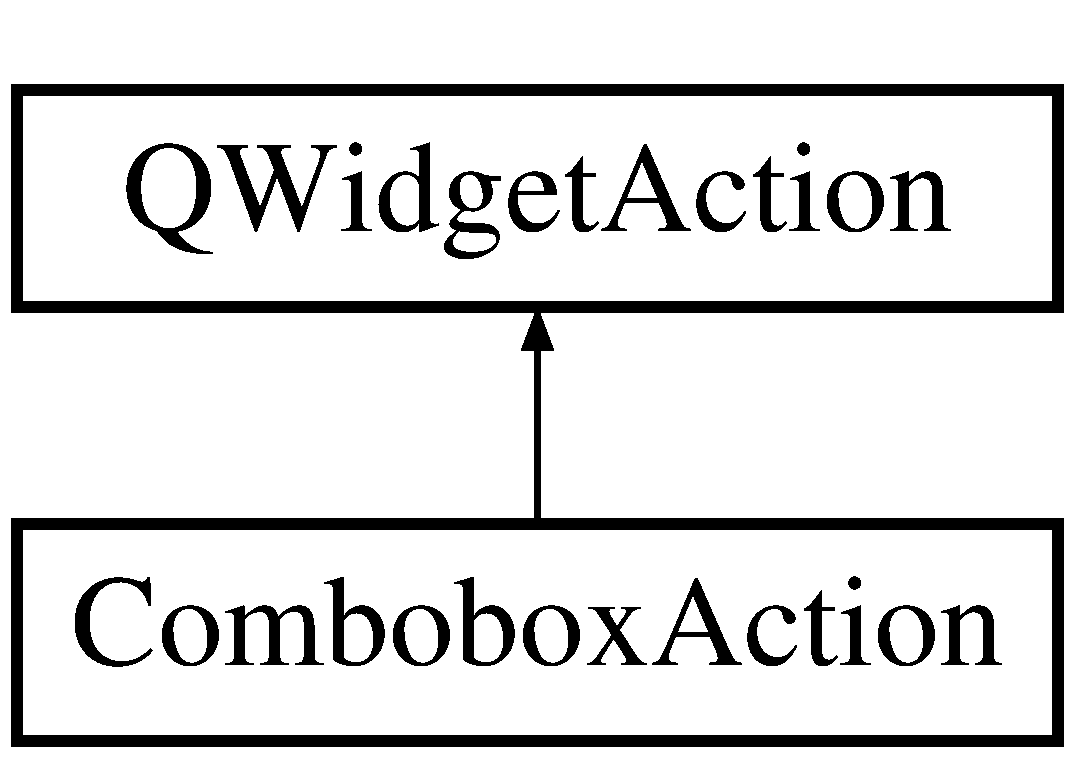
\includegraphics[height=2.000000cm]{classComboboxAction}
\end{center}
\end{figure}
\subsection*{Public Member Functions}
\begin{DoxyCompactItemize}
\item 
\mbox{\Hypertarget{classComboboxAction_afa2a6bfade094a82beef7d478c5a4cf8}\label{classComboboxAction_afa2a6bfade094a82beef7d478c5a4cf8}} 
{\bfseries Combobox\+Action} (const Q\+String \&info)
\item 
\mbox{\Hypertarget{classComboboxAction_adfe475154e5b88eddbc9a51759bdf312}\label{classComboboxAction_adfe475154e5b88eddbc9a51759bdf312}} 
int {\bfseries Combo\+Index} ()
\end{DoxyCompactItemize}


\subsection{Detailed Description}


Definition at line 13 of file combobox\+\_\+action.\+hpp.



The documentation for this class was generated from the following files\+:\begin{DoxyCompactItemize}
\item 
include/combobox\+\_\+action.\+hpp\item 
src/combobox\+\_\+action.\+cpp\end{DoxyCompactItemize}

\hypertarget{classGUI}{}\section{G\+UI Class Reference}
\label{classGUI}\index{G\+UI@{G\+UI}}


Graphical user interface.  




{\ttfamily \#include $<$gui.\+hpp$>$}

Inheritance diagram for G\+UI\+:\begin{figure}[H]
\begin{center}
\leavevmode
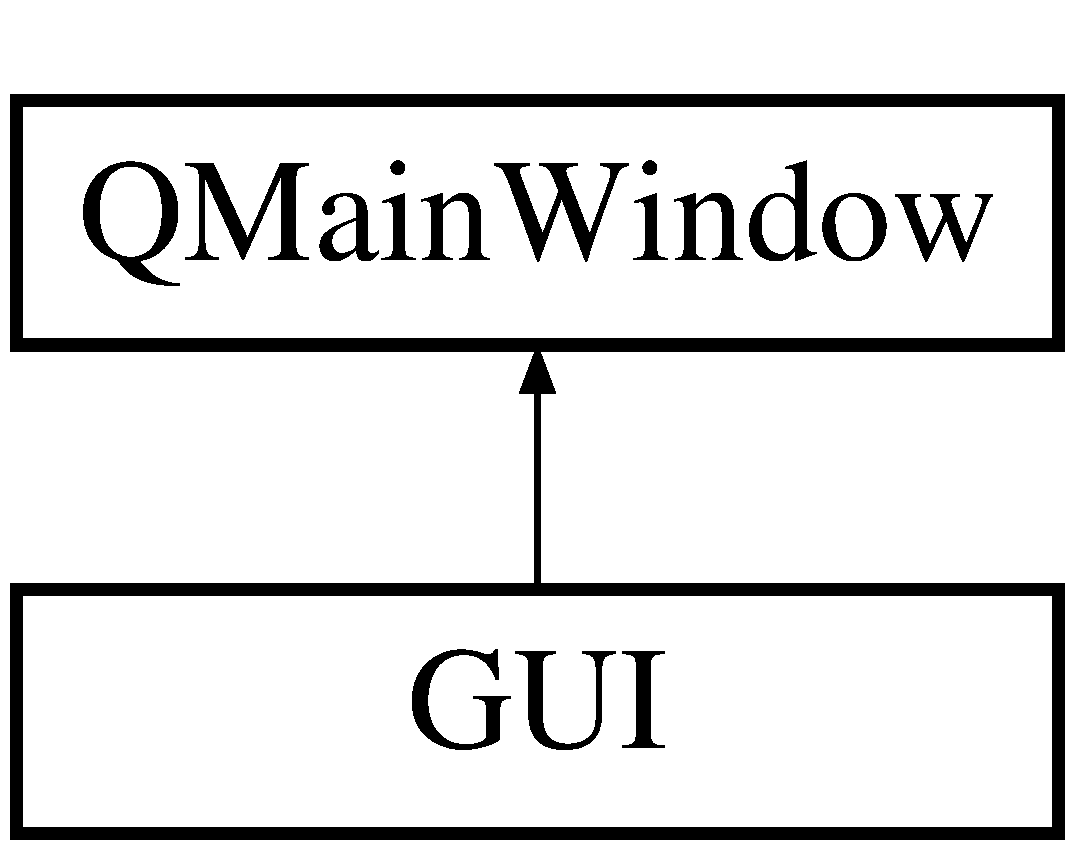
\includegraphics[height=2.000000cm]{classGUI}
\end{center}
\end{figure}
\subsection*{Public Member Functions}
\begin{DoxyCompactItemize}
\item 
\mbox{\hyperlink{classGUI_acb0ba8c6fc121d814d30560e2c29f2fe}{G\+UI}} (Q\+Widget $\ast$parent=0)
\begin{DoxyCompactList}\small\item\em \mbox{\hyperlink{classGUI}{G\+UI}} constructor. \end{DoxyCompactList}\item 
\mbox{\hyperlink{classGUI_ac9cae2328dcb5d83bdfaeca49a2eb695}{$\sim$\+G\+UI}} ()
\begin{DoxyCompactList}\small\item\em \mbox{\hyperlink{classGUI}{G\+UI}} deconstructor. \end{DoxyCompactList}\item 
void \mbox{\hyperlink{classGUI_a91fab5d31617ad5631d17dfceb5a0fad}{Line\+Mode}} ()
\begin{DoxyCompactList}\small\item\em Line drawing mode. \end{DoxyCompactList}\item 
void \mbox{\hyperlink{classGUI_aac66154aaa763aac4d20e55cbd1bdc0d}{Delete\+Mode}} ()
\begin{DoxyCompactList}\small\item\em Delete lines mode. \end{DoxyCompactList}\item 
void \mbox{\hyperlink{classGUI_afb6e169c9372800e69c70a3889420325}{Clear\+Mode}} ()
\begin{DoxyCompactList}\small\item\em Clear previous points. \end{DoxyCompactList}\item 
void \mbox{\hyperlink{classGUI_a19c82a62a2b41460c81317fa967e3a1e}{Clear\+All}} ()
\begin{DoxyCompactList}\small\item\em Clear all objects. \end{DoxyCompactList}\item 
void \mbox{\hyperlink{classGUI_a44684af7706c021022520e2c4829c3ee}{save\+Image}} ()
\begin{DoxyCompactList}\small\item\em Save scene content to an image. \end{DoxyCompactList}\item 
void \mbox{\hyperlink{classGUI_a925c89bd7b32ccc8d726063ed8076f8f}{open\+Image}} ()
\begin{DoxyCompactList}\small\item\em Open an image. \end{DoxyCompactList}\item 
void \mbox{\hyperlink{classGUI_a5281fa4256d3ff14df9a95c1c6613bb2}{Img\+Mode}} ()
\begin{DoxyCompactList}\small\item\em Mode for adding images to the scene. \end{DoxyCompactList}\item 
void \mbox{\hyperlink{classGUI_a453b758a292b4a0e6f52f25b1bb2de77}{Delete\+Img\+Mode}} ()
\begin{DoxyCompactList}\small\item\em Delete images from the scene. \end{DoxyCompactList}\item 
void \mbox{\hyperlink{classGUI_ae8acfcce2ea4da241c920076b72f1c93}{Cut\+Image\+Mode}} ()
\begin{DoxyCompactList}\small\item\em Mode for cutting images. \end{DoxyCompactList}\item 
void \mbox{\hyperlink{classGUI_a26cdc4a989f3637301f0afb9cc5e23b0}{create\+Toolbars}} ()
\begin{DoxyCompactList}\small\item\em Create different toolbars. \end{DoxyCompactList}\item 
void \mbox{\hyperlink{classGUI_aaf633cd0904e4c3627c21219f330c177}{Hide\+Polygon\+Toolbar}} (bool hide)
\begin{DoxyCompactList}\small\item\em Hide \mbox{\hyperlink{structPolygonToolbar}{Polygon\+Toolbar}}. \end{DoxyCompactList}\item 
void \mbox{\hyperlink{classGUI_a9517c0ad1e4c2b39faab8050f8133151}{Hide\+Mode\+Toolbar}} (bool hide)
\begin{DoxyCompactList}\small\item\em Hide \mbox{\hyperlink{structModeToolbar}{Mode\+Toolbar}}. \end{DoxyCompactList}\item 
void \mbox{\hyperlink{classGUI_aa115b0163bfbf518dd201f4f02476b75}{Hide\+Main\+Toolbar}} (bool hide)
\begin{DoxyCompactList}\small\item\em Hide Main\+Toolbar. \end{DoxyCompactList}\item 
void \mbox{\hyperlink{classGUI_a7f6d3b1fcbd874fccd93c5f29c468ed8}{Hide\+Select\+Toolbar}} (bool hide)
\begin{DoxyCompactList}\small\item\em Hide \mbox{\hyperlink{structSelectImgToolbar}{Select\+Img\+Toolbar}}. \end{DoxyCompactList}\item 
void \mbox{\hyperlink{classGUI_a3547730e0fae81b59fcb19d00a370782}{Continue\+From\+Mode}} ()
\begin{DoxyCompactList}\small\item\em Continue to image cutting. \end{DoxyCompactList}\item 
void \mbox{\hyperlink{classGUI_a8188dd01b2dc9354afbbf2f4b18fd19a}{Cancel\+From\+Mode}} ()
\begin{DoxyCompactList}\small\item\em Cancel to the main view, toolbar. \end{DoxyCompactList}\item 
void \mbox{\hyperlink{classGUI_a6bf2d3ef382340365b5693245a2bd955}{Set\+Poly\+Final}} ()
\begin{DoxyCompactList}\small\item\em Create polygon cut to an image. \end{DoxyCompactList}\item 
void \mbox{\hyperlink{classGUI_abf8e1050ae4d599bf35af7b1f841d960}{Remove\+Poly\+Previous}} ()
\begin{DoxyCompactList}\small\item\em Remove previous cut line from an image. \end{DoxyCompactList}\item 
void \mbox{\hyperlink{classGUI_a9f2b3abf533a7c720b817caed653da2e}{Cancel\+From\+Poly}} ()
\begin{DoxyCompactList}\small\item\em Return to the main view. \end{DoxyCompactList}\item 
void \mbox{\hyperlink{classGUI_a0cddf3859f457495040857f4868f32e3}{Continue\+From\+Select}} ()
\begin{DoxyCompactList}\small\item\em Continue to image mode select. \end{DoxyCompactList}\item 
void \mbox{\hyperlink{classGUI_a3e6d9c2c9482bf8cb9655899b36e8bc1}{Cancel\+From\+Select}} ()
\begin{DoxyCompactList}\small\item\em Return to the main view. \end{DoxyCompactList}\item 
void \mbox{\hyperlink{classGUI_a00fb847ea0a8249acaaf70c0f3ba3fd4}{Save\+Choices}} ()
\begin{DoxyCompactList}\small\item\em Save options. \end{DoxyCompactList}\item 
\mbox{\Hypertarget{classGUI_ac0cb178a0a36573f7d99a104dd84f5ed}\label{classGUI_ac0cb178a0a36573f7d99a104dd84f5ed}} 
void \mbox{\hyperlink{classGUI_ac0cb178a0a36573f7d99a104dd84f5ed}{Bezier\+Mode}} ()
\begin{DoxyCompactList}\small\item\em Activates/deactivates bezier\+\_\+mode. \end{DoxyCompactList}\item 
void \mbox{\hyperlink{classGUI_a593ffaac7d8a664f20893aed2536988b}{Bezier\+Toolbar\+\_\+\+Options\+Saved}} ()
\begin{DoxyCompactList}\small\item\em Driggered when \mbox{\hyperlink{structBezierToolbar}{Bezier\+Toolbar}} options are saved. \end{DoxyCompactList}\item 
void \mbox{\hyperlink{classGUI_a6f27f73cf15f18dfa206630cc77bc7df}{Bezier\+Toolbar\+\_\+\+Save\+Bezier}} ()
\begin{DoxyCompactList}\small\item\em Save the current \mbox{\hyperlink{classBezier}{Bezier}}. \end{DoxyCompactList}\item 
\mbox{\Hypertarget{classGUI_a8e851696d9c01c19a3afc7bdc0fbe54f}\label{classGUI_a8e851696d9c01c19a3afc7bdc0fbe54f}} 
void \mbox{\hyperlink{classGUI_a8e851696d9c01c19a3afc7bdc0fbe54f}{Bezier\+Toolbar\+\_\+\+Cancel}} ()
\begin{DoxyCompactList}\small\item\em Remove the current \mbox{\hyperlink{classBezier}{Bezier}} and cancel to main toolbar. \end{DoxyCompactList}\item 
\mbox{\Hypertarget{classGUI_a508f3c222bb40b6cf139fc346e562564}\label{classGUI_a508f3c222bb40b6cf139fc346e562564}} 
void \mbox{\hyperlink{classGUI_a508f3c222bb40b6cf139fc346e562564}{Bezier\+Toolbar\+\_\+\+Remove}} ()
\begin{DoxyCompactList}\small\item\em Remove current \mbox{\hyperlink{classBezier}{Bezier}}. \end{DoxyCompactList}\item 
void \mbox{\hyperlink{classGUI_ae36c91ff70502eeecb985c3b84aa3a07}{Hide\+Bezier\+Toolbar}} (bool hide)
\begin{DoxyCompactList}\small\item\em Hide or unhide \mbox{\hyperlink{structBezierToolbar}{Bezier\+Toolbar}}. \end{DoxyCompactList}\end{DoxyCompactItemize}


\subsection{Detailed Description}
Graphical user interface. 

Inherits Q\+Main\+Window. Implements inteface to mainwidget 

Definition at line 188 of file gui.\+hpp.



\subsection{Constructor \& Destructor Documentation}
\mbox{\Hypertarget{classGUI_acb0ba8c6fc121d814d30560e2c29f2fe}\label{classGUI_acb0ba8c6fc121d814d30560e2c29f2fe}} 
\index{G\+UI@{G\+UI}!G\+UI@{G\+UI}}
\index{G\+UI@{G\+UI}!G\+UI@{G\+UI}}
\subsubsection{\texorpdfstring{G\+U\+I()}{GUI()}}
{\footnotesize\ttfamily G\+U\+I\+::\+G\+UI (\begin{DoxyParamCaption}\item[{Q\+Widget $\ast$}]{parent = {\ttfamily 0} }\end{DoxyParamCaption})}



\mbox{\hyperlink{classGUI}{G\+UI}} constructor. 


\begin{DoxyParams}{Parameters}
{\em parent} & the parent widget \\
\hline
\end{DoxyParams}


Definition at line 17 of file gui.\+cpp.

\mbox{\Hypertarget{classGUI_ac9cae2328dcb5d83bdfaeca49a2eb695}\label{classGUI_ac9cae2328dcb5d83bdfaeca49a2eb695}} 
\index{G\+UI@{G\+UI}!````~G\+UI@{$\sim$\+G\+UI}}
\index{````~G\+UI@{$\sim$\+G\+UI}!G\+UI@{G\+UI}}
\subsubsection{\texorpdfstring{$\sim$\+G\+U\+I()}{~GUI()}}
{\footnotesize\ttfamily G\+U\+I\+::$\sim$\+G\+UI (\begin{DoxyParamCaption}{ }\end{DoxyParamCaption})\hspace{0.3cm}{\ttfamily [inline]}}



\mbox{\hyperlink{classGUI}{G\+UI}} deconstructor. 

Deletes mainwidget 

Definition at line 202 of file gui.\+hpp.



\subsection{Member Function Documentation}
\mbox{\Hypertarget{classGUI_a593ffaac7d8a664f20893aed2536988b}\label{classGUI_a593ffaac7d8a664f20893aed2536988b}} 
\index{G\+UI@{G\+UI}!Bezier\+Toolbar\+\_\+\+Options\+Saved@{Bezier\+Toolbar\+\_\+\+Options\+Saved}}
\index{Bezier\+Toolbar\+\_\+\+Options\+Saved@{Bezier\+Toolbar\+\_\+\+Options\+Saved}!G\+UI@{G\+UI}}
\subsubsection{\texorpdfstring{Bezier\+Toolbar\+\_\+\+Options\+Saved()}{BezierToolbar\_OptionsSaved()}}
{\footnotesize\ttfamily void G\+U\+I\+::\+Bezier\+Toolbar\+\_\+\+Options\+Saved (\begin{DoxyParamCaption}{ }\end{DoxyParamCaption})}



Driggered when \mbox{\hyperlink{structBezierToolbar}{Bezier\+Toolbar}} options are saved. 

Used to update \mbox{\hyperlink{classOwnGraphicsScene}{Own\+Graphics\+Scene}} \mbox{\hyperlink{classBezier}{Bezier}} drawing 

Definition at line 685 of file gui.\+cpp.

\mbox{\Hypertarget{classGUI_a6f27f73cf15f18dfa206630cc77bc7df}\label{classGUI_a6f27f73cf15f18dfa206630cc77bc7df}} 
\index{G\+UI@{G\+UI}!Bezier\+Toolbar\+\_\+\+Save\+Bezier@{Bezier\+Toolbar\+\_\+\+Save\+Bezier}}
\index{Bezier\+Toolbar\+\_\+\+Save\+Bezier@{Bezier\+Toolbar\+\_\+\+Save\+Bezier}!G\+UI@{G\+UI}}
\subsubsection{\texorpdfstring{Bezier\+Toolbar\+\_\+\+Save\+Bezier()}{BezierToolbar\_SaveBezier()}}
{\footnotesize\ttfamily void G\+U\+I\+::\+Bezier\+Toolbar\+\_\+\+Save\+Bezier (\begin{DoxyParamCaption}{ }\end{DoxyParamCaption})}



Save the current \mbox{\hyperlink{classBezier}{Bezier}}. 

Used to signal \mbox{\hyperlink{classOwnGraphicsScene}{Own\+Graphics\+Scene}} that the \mbox{\hyperlink{classBezier}{Bezier}} should be saved 

Definition at line 703 of file gui.\+cpp.

\mbox{\Hypertarget{classGUI_a8188dd01b2dc9354afbbf2f4b18fd19a}\label{classGUI_a8188dd01b2dc9354afbbf2f4b18fd19a}} 
\index{G\+UI@{G\+UI}!Cancel\+From\+Mode@{Cancel\+From\+Mode}}
\index{Cancel\+From\+Mode@{Cancel\+From\+Mode}!G\+UI@{G\+UI}}
\subsubsection{\texorpdfstring{Cancel\+From\+Mode()}{CancelFromMode()}}
{\footnotesize\ttfamily void G\+U\+I\+::\+Cancel\+From\+Mode (\begin{DoxyParamCaption}{ }\end{DoxyParamCaption})}



Cancel to the main view, toolbar. 

Called after user has canceled from image cutting mode 

Definition at line 573 of file gui.\+cpp.

\mbox{\Hypertarget{classGUI_a9f2b3abf533a7c720b817caed653da2e}\label{classGUI_a9f2b3abf533a7c720b817caed653da2e}} 
\index{G\+UI@{G\+UI}!Cancel\+From\+Poly@{Cancel\+From\+Poly}}
\index{Cancel\+From\+Poly@{Cancel\+From\+Poly}!G\+UI@{G\+UI}}
\subsubsection{\texorpdfstring{Cancel\+From\+Poly()}{CancelFromPoly()}}
{\footnotesize\ttfamily void G\+U\+I\+::\+Cancel\+From\+Poly (\begin{DoxyParamCaption}{ }\end{DoxyParamCaption})}



Return to the main view. 

Called after user has canceled from polygon image cut 

Definition at line 618 of file gui.\+cpp.

\mbox{\Hypertarget{classGUI_a3e6d9c2c9482bf8cb9655899b36e8bc1}\label{classGUI_a3e6d9c2c9482bf8cb9655899b36e8bc1}} 
\index{G\+UI@{G\+UI}!Cancel\+From\+Select@{Cancel\+From\+Select}}
\index{Cancel\+From\+Select@{Cancel\+From\+Select}!G\+UI@{G\+UI}}
\subsubsection{\texorpdfstring{Cancel\+From\+Select()}{CancelFromSelect()}}
{\footnotesize\ttfamily void G\+U\+I\+::\+Cancel\+From\+Select (\begin{DoxyParamCaption}{ }\end{DoxyParamCaption})}



Return to the main view. 

Called after user has canceled from image select 

Definition at line 534 of file gui.\+cpp.

\mbox{\Hypertarget{classGUI_a19c82a62a2b41460c81317fa967e3a1e}\label{classGUI_a19c82a62a2b41460c81317fa967e3a1e}} 
\index{G\+UI@{G\+UI}!Clear\+All@{Clear\+All}}
\index{Clear\+All@{Clear\+All}!G\+UI@{G\+UI}}
\subsubsection{\texorpdfstring{Clear\+All()}{ClearAll()}}
{\footnotesize\ttfamily void G\+U\+I\+::\+Clear\+All (\begin{DoxyParamCaption}{ }\end{DoxyParamCaption})}



Clear all objects. 

User triggered Q\+Action sends a signal and clears all 

Definition at line 149 of file gui.\+cpp.

\mbox{\Hypertarget{classGUI_afb6e169c9372800e69c70a3889420325}\label{classGUI_afb6e169c9372800e69c70a3889420325}} 
\index{G\+UI@{G\+UI}!Clear\+Mode@{Clear\+Mode}}
\index{Clear\+Mode@{Clear\+Mode}!G\+UI@{G\+UI}}
\subsubsection{\texorpdfstring{Clear\+Mode()}{ClearMode()}}
{\footnotesize\ttfamily void G\+U\+I\+::\+Clear\+Mode (\begin{DoxyParamCaption}{ }\end{DoxyParamCaption})}



Clear previous points. 

Triggers clear mode in the scene 

Definition at line 143 of file gui.\+cpp.

\mbox{\Hypertarget{classGUI_a3547730e0fae81b59fcb19d00a370782}\label{classGUI_a3547730e0fae81b59fcb19d00a370782}} 
\index{G\+UI@{G\+UI}!Continue\+From\+Mode@{Continue\+From\+Mode}}
\index{Continue\+From\+Mode@{Continue\+From\+Mode}!G\+UI@{G\+UI}}
\subsubsection{\texorpdfstring{Continue\+From\+Mode()}{ContinueFromMode()}}
{\footnotesize\ttfamily void G\+U\+I\+::\+Continue\+From\+Mode (\begin{DoxyParamCaption}{ }\end{DoxyParamCaption})}



Continue to image cutting. 

Called after user has selected image cutting mode 

Definition at line 586 of file gui.\+cpp.

\mbox{\Hypertarget{classGUI_a0cddf3859f457495040857f4868f32e3}\label{classGUI_a0cddf3859f457495040857f4868f32e3}} 
\index{G\+UI@{G\+UI}!Continue\+From\+Select@{Continue\+From\+Select}}
\index{Continue\+From\+Select@{Continue\+From\+Select}!G\+UI@{G\+UI}}
\subsubsection{\texorpdfstring{Continue\+From\+Select()}{ContinueFromSelect()}}
{\footnotesize\ttfamily void G\+U\+I\+::\+Continue\+From\+Select (\begin{DoxyParamCaption}{ }\end{DoxyParamCaption})}



Continue to image mode select. 

Called after user has selected which image to cut 

Definition at line 550 of file gui.\+cpp.

\mbox{\Hypertarget{classGUI_a26cdc4a989f3637301f0afb9cc5e23b0}\label{classGUI_a26cdc4a989f3637301f0afb9cc5e23b0}} 
\index{G\+UI@{G\+UI}!create\+Toolbars@{create\+Toolbars}}
\index{create\+Toolbars@{create\+Toolbars}!G\+UI@{G\+UI}}
\subsubsection{\texorpdfstring{create\+Toolbars()}{createToolbars()}}
{\footnotesize\ttfamily void G\+U\+I\+::create\+Toolbars (\begin{DoxyParamCaption}{ }\end{DoxyParamCaption})}



Create different toolbars. 

Called from \mbox{\hyperlink{classGUI}{G\+UI}} constructor to create all toolbars 

Definition at line 354 of file gui.\+cpp.

\mbox{\Hypertarget{classGUI_ae8acfcce2ea4da241c920076b72f1c93}\label{classGUI_ae8acfcce2ea4da241c920076b72f1c93}} 
\index{G\+UI@{G\+UI}!Cut\+Image\+Mode@{Cut\+Image\+Mode}}
\index{Cut\+Image\+Mode@{Cut\+Image\+Mode}!G\+UI@{G\+UI}}
\subsubsection{\texorpdfstring{Cut\+Image\+Mode()}{CutImageMode()}}
{\footnotesize\ttfamily void G\+U\+I\+::\+Cut\+Image\+Mode (\begin{DoxyParamCaption}{ }\end{DoxyParamCaption})}



Mode for cutting images. 

Images can be cut to multiple shapes. Starts a toolbar which promts user to choose which image is being cut. Then user chooses cut style and finally cuts the image 

Definition at line 263 of file gui.\+cpp.

\mbox{\Hypertarget{classGUI_a453b758a292b4a0e6f52f25b1bb2de77}\label{classGUI_a453b758a292b4a0e6f52f25b1bb2de77}} 
\index{G\+UI@{G\+UI}!Delete\+Img\+Mode@{Delete\+Img\+Mode}}
\index{Delete\+Img\+Mode@{Delete\+Img\+Mode}!G\+UI@{G\+UI}}
\subsubsection{\texorpdfstring{Delete\+Img\+Mode()}{DeleteImgMode()}}
{\footnotesize\ttfamily void G\+U\+I\+::\+Delete\+Img\+Mode (\begin{DoxyParamCaption}{ }\end{DoxyParamCaption})}



Delete images from the scene. 

User holds cursor over an image and clicks to delete the image 

Definition at line 244 of file gui.\+cpp.

\mbox{\Hypertarget{classGUI_aac66154aaa763aac4d20e55cbd1bdc0d}\label{classGUI_aac66154aaa763aac4d20e55cbd1bdc0d}} 
\index{G\+UI@{G\+UI}!Delete\+Mode@{Delete\+Mode}}
\index{Delete\+Mode@{Delete\+Mode}!G\+UI@{G\+UI}}
\subsubsection{\texorpdfstring{Delete\+Mode()}{DeleteMode()}}
{\footnotesize\ttfamily void G\+U\+I\+::\+Delete\+Mode (\begin{DoxyParamCaption}{ }\end{DoxyParamCaption})}



Delete lines mode. 

Q\+Action sends a signal and activates or deactivates delete mode 

Definition at line 123 of file gui.\+cpp.

\mbox{\Hypertarget{classGUI_ae36c91ff70502eeecb985c3b84aa3a07}\label{classGUI_ae36c91ff70502eeecb985c3b84aa3a07}} 
\index{G\+UI@{G\+UI}!Hide\+Bezier\+Toolbar@{Hide\+Bezier\+Toolbar}}
\index{Hide\+Bezier\+Toolbar@{Hide\+Bezier\+Toolbar}!G\+UI@{G\+UI}}
\subsubsection{\texorpdfstring{Hide\+Bezier\+Toolbar()}{HideBezierToolbar()}}
{\footnotesize\ttfamily void G\+U\+I\+::\+Hide\+Bezier\+Toolbar (\begin{DoxyParamCaption}\item[{bool}]{hide }\end{DoxyParamCaption})}



Hide or unhide \mbox{\hyperlink{structBezierToolbar}{Bezier\+Toolbar}}. 


\begin{DoxyParams}{Parameters}
{\em hide} & true -\/$>$ hide, false -\/$>$ unhide \\
\hline
\end{DoxyParams}


Definition at line 725 of file gui.\+cpp.

\mbox{\Hypertarget{classGUI_aa115b0163bfbf518dd201f4f02476b75}\label{classGUI_aa115b0163bfbf518dd201f4f02476b75}} 
\index{G\+UI@{G\+UI}!Hide\+Main\+Toolbar@{Hide\+Main\+Toolbar}}
\index{Hide\+Main\+Toolbar@{Hide\+Main\+Toolbar}!G\+UI@{G\+UI}}
\subsubsection{\texorpdfstring{Hide\+Main\+Toolbar()}{HideMainToolbar()}}
{\footnotesize\ttfamily void G\+U\+I\+::\+Hide\+Main\+Toolbar (\begin{DoxyParamCaption}\item[{bool}]{hide }\end{DoxyParamCaption})}



Hide Main\+Toolbar. 


\begin{DoxyParams}{Parameters}
{\em hide} & if true hides the toolbar \\
\hline
\end{DoxyParams}


Definition at line 323 of file gui.\+cpp.

\mbox{\Hypertarget{classGUI_a9517c0ad1e4c2b39faab8050f8133151}\label{classGUI_a9517c0ad1e4c2b39faab8050f8133151}} 
\index{G\+UI@{G\+UI}!Hide\+Mode\+Toolbar@{Hide\+Mode\+Toolbar}}
\index{Hide\+Mode\+Toolbar@{Hide\+Mode\+Toolbar}!G\+UI@{G\+UI}}
\subsubsection{\texorpdfstring{Hide\+Mode\+Toolbar()}{HideModeToolbar()}}
{\footnotesize\ttfamily void G\+U\+I\+::\+Hide\+Mode\+Toolbar (\begin{DoxyParamCaption}\item[{bool}]{hide }\end{DoxyParamCaption})}



Hide \mbox{\hyperlink{structModeToolbar}{Mode\+Toolbar}}. 


\begin{DoxyParams}{Parameters}
{\em hide} & if true hides the toolbar \\
\hline
\end{DoxyParams}


Definition at line 308 of file gui.\+cpp.

\mbox{\Hypertarget{classGUI_aaf633cd0904e4c3627c21219f330c177}\label{classGUI_aaf633cd0904e4c3627c21219f330c177}} 
\index{G\+UI@{G\+UI}!Hide\+Polygon\+Toolbar@{Hide\+Polygon\+Toolbar}}
\index{Hide\+Polygon\+Toolbar@{Hide\+Polygon\+Toolbar}!G\+UI@{G\+UI}}
\subsubsection{\texorpdfstring{Hide\+Polygon\+Toolbar()}{HidePolygonToolbar()}}
{\footnotesize\ttfamily void G\+U\+I\+::\+Hide\+Polygon\+Toolbar (\begin{DoxyParamCaption}\item[{bool}]{hide }\end{DoxyParamCaption})}



Hide \mbox{\hyperlink{structPolygonToolbar}{Polygon\+Toolbar}}. 


\begin{DoxyParams}{Parameters}
{\em hide} & if true hides the toolbar \\
\hline
\end{DoxyParams}


Definition at line 293 of file gui.\+cpp.

\mbox{\Hypertarget{classGUI_a7f6d3b1fcbd874fccd93c5f29c468ed8}\label{classGUI_a7f6d3b1fcbd874fccd93c5f29c468ed8}} 
\index{G\+UI@{G\+UI}!Hide\+Select\+Toolbar@{Hide\+Select\+Toolbar}}
\index{Hide\+Select\+Toolbar@{Hide\+Select\+Toolbar}!G\+UI@{G\+UI}}
\subsubsection{\texorpdfstring{Hide\+Select\+Toolbar()}{HideSelectToolbar()}}
{\footnotesize\ttfamily void G\+U\+I\+::\+Hide\+Select\+Toolbar (\begin{DoxyParamCaption}\item[{bool}]{hide }\end{DoxyParamCaption})}



Hide \mbox{\hyperlink{structSelectImgToolbar}{Select\+Img\+Toolbar}}. 


\begin{DoxyParams}{Parameters}
{\em hide} & if true hides the toolbar \\
\hline
\end{DoxyParams}


Definition at line 337 of file gui.\+cpp.

\mbox{\Hypertarget{classGUI_a5281fa4256d3ff14df9a95c1c6613bb2}\label{classGUI_a5281fa4256d3ff14df9a95c1c6613bb2}} 
\index{G\+UI@{G\+UI}!Img\+Mode@{Img\+Mode}}
\index{Img\+Mode@{Img\+Mode}!G\+UI@{G\+UI}}
\subsubsection{\texorpdfstring{Img\+Mode()}{ImgMode()}}
{\footnotesize\ttfamily void G\+U\+I\+::\+Img\+Mode (\begin{DoxyParamCaption}{ }\end{DoxyParamCaption})}



Mode for adding images to the scene. 

User can drag image and then save it to the scene 

Definition at line 216 of file gui.\+cpp.

\mbox{\Hypertarget{classGUI_a91fab5d31617ad5631d17dfceb5a0fad}\label{classGUI_a91fab5d31617ad5631d17dfceb5a0fad}} 
\index{G\+UI@{G\+UI}!Line\+Mode@{Line\+Mode}}
\index{Line\+Mode@{Line\+Mode}!G\+UI@{G\+UI}}
\subsubsection{\texorpdfstring{Line\+Mode()}{LineMode()}}
{\footnotesize\ttfamily void G\+U\+I\+::\+Line\+Mode (\begin{DoxyParamCaption}{ }\end{DoxyParamCaption})}



Line drawing mode. 

Q\+Action sends a signal and activates or deactivates line mode 

Definition at line 104 of file gui.\+cpp.

\mbox{\Hypertarget{classGUI_a925c89bd7b32ccc8d726063ed8076f8f}\label{classGUI_a925c89bd7b32ccc8d726063ed8076f8f}} 
\index{G\+UI@{G\+UI}!open\+Image@{open\+Image}}
\index{open\+Image@{open\+Image}!G\+UI@{G\+UI}}
\subsubsection{\texorpdfstring{open\+Image()}{openImage()}}
{\footnotesize\ttfamily void G\+U\+I\+::open\+Image (\begin{DoxyParamCaption}{ }\end{DoxyParamCaption})}



Open an image. 

By activating image mode user can place the image to the scene 

Definition at line 195 of file gui.\+cpp.

\mbox{\Hypertarget{classGUI_abf8e1050ae4d599bf35af7b1f841d960}\label{classGUI_abf8e1050ae4d599bf35af7b1f841d960}} 
\index{G\+UI@{G\+UI}!Remove\+Poly\+Previous@{Remove\+Poly\+Previous}}
\index{Remove\+Poly\+Previous@{Remove\+Poly\+Previous}!G\+UI@{G\+UI}}
\subsubsection{\texorpdfstring{Remove\+Poly\+Previous()}{RemovePolyPrevious()}}
{\footnotesize\ttfamily void G\+U\+I\+::\+Remove\+Poly\+Previous (\begin{DoxyParamCaption}{ }\end{DoxyParamCaption})}



Remove previous cut line from an image. 

Triggered by user action 

Definition at line 648 of file gui.\+cpp.

\mbox{\Hypertarget{classGUI_a00fb847ea0a8249acaaf70c0f3ba3fd4}\label{classGUI_a00fb847ea0a8249acaaf70c0f3ba3fd4}} 
\index{G\+UI@{G\+UI}!Save\+Choices@{Save\+Choices}}
\index{Save\+Choices@{Save\+Choices}!G\+UI@{G\+UI}}
\subsubsection{\texorpdfstring{Save\+Choices()}{SaveChoices()}}
{\footnotesize\ttfamily void G\+U\+I\+::\+Save\+Choices (\begin{DoxyParamCaption}{ }\end{DoxyParamCaption})}



Save options. 

Called after user has modified options combobox and wants to save the options 

Definition at line 657 of file gui.\+cpp.

\mbox{\Hypertarget{classGUI_a44684af7706c021022520e2c4829c3ee}\label{classGUI_a44684af7706c021022520e2c4829c3ee}} 
\index{G\+UI@{G\+UI}!save\+Image@{save\+Image}}
\index{save\+Image@{save\+Image}!G\+UI@{G\+UI}}
\subsubsection{\texorpdfstring{save\+Image()}{saveImage()}}
{\footnotesize\ttfamily void G\+U\+I\+::save\+Image (\begin{DoxyParamCaption}{ }\end{DoxyParamCaption})}



Save scene content to an image. 

User can specify where the image is saved 

Definition at line 156 of file gui.\+cpp.

\mbox{\Hypertarget{classGUI_a6bf2d3ef382340365b5693245a2bd955}\label{classGUI_a6bf2d3ef382340365b5693245a2bd955}} 
\index{G\+UI@{G\+UI}!Set\+Poly\+Final@{Set\+Poly\+Final}}
\index{Set\+Poly\+Final@{Set\+Poly\+Final}!G\+UI@{G\+UI}}
\subsubsection{\texorpdfstring{Set\+Poly\+Final()}{SetPolyFinal()}}
{\footnotesize\ttfamily void G\+U\+I\+::\+Set\+Poly\+Final (\begin{DoxyParamCaption}{ }\end{DoxyParamCaption})}



Create polygon cut to an image. 

Triggered by user when user is ready to cut the image 

Definition at line 634 of file gui.\+cpp.



The documentation for this class was generated from the following files\+:\begin{DoxyCompactItemize}
\item 
include/\mbox{\hyperlink{gui_8hpp}{gui.\+hpp}}\item 
src/\mbox{\hyperlink{gui_8cpp}{gui.\+cpp}}\end{DoxyCompactItemize}

\hypertarget{structImage__Active}{}\section{Image\+\_\+\+Active Struct Reference}
\label{structImage__Active}\index{Image\+\_\+\+Active@{Image\+\_\+\+Active}}


Contains active image.  




{\ttfamily \#include $<$Own\+Graphics\+Scene.\+hpp$>$}

\subsection*{Public Attributes}
\begin{DoxyCompactItemize}
\item 
bool \mbox{\hyperlink{structImage__Active_ac5eb10f5ca4ad81766c92a6ede6f7853}{added\+\_\+scene}} = false
\item 
\mbox{\hyperlink{classPixmapItem}{Pixmap\+Item}} $\ast$ \mbox{\hyperlink{structImage__Active_aa007ea3c9ba4830bbc2706af51820c20}{pixmap\+\_\+item}}
\item 
unsigned char \mbox{\hyperlink{structImage__Active_abb039226daf0372a8d88c842f5eb140f}{clicks}} = 0
\end{DoxyCompactItemize}


\subsection{Detailed Description}
Contains active image. 

Used to when user is in image\+\_\+mode 

Definition at line 53 of file Own\+Graphics\+Scene.\+hpp.



\subsection{Member Data Documentation}
\mbox{\Hypertarget{structImage__Active_ac5eb10f5ca4ad81766c92a6ede6f7853}\label{structImage__Active_ac5eb10f5ca4ad81766c92a6ede6f7853}} 
\index{Image\+\_\+\+Active@{Image\+\_\+\+Active}!added\+\_\+scene@{added\+\_\+scene}}
\index{added\+\_\+scene@{added\+\_\+scene}!Image\+\_\+\+Active@{Image\+\_\+\+Active}}
\subsubsection{\texorpdfstring{added\+\_\+scene}{added\_scene}}
{\footnotesize\ttfamily bool Image\+\_\+\+Active\+::added\+\_\+scene = false}

Is image added to scene 

Definition at line 56 of file Own\+Graphics\+Scene.\+hpp.

\mbox{\Hypertarget{structImage__Active_abb039226daf0372a8d88c842f5eb140f}\label{structImage__Active_abb039226daf0372a8d88c842f5eb140f}} 
\index{Image\+\_\+\+Active@{Image\+\_\+\+Active}!clicks@{clicks}}
\index{clicks@{clicks}!Image\+\_\+\+Active@{Image\+\_\+\+Active}}
\subsubsection{\texorpdfstring{clicks}{clicks}}
{\footnotesize\ttfamily unsigned char Image\+\_\+\+Active\+::clicks = 0}

Counter for mouse clicks 

Definition at line 58 of file Own\+Graphics\+Scene.\+hpp.

\mbox{\Hypertarget{structImage__Active_aa007ea3c9ba4830bbc2706af51820c20}\label{structImage__Active_aa007ea3c9ba4830bbc2706af51820c20}} 
\index{Image\+\_\+\+Active@{Image\+\_\+\+Active}!pixmap\+\_\+item@{pixmap\+\_\+item}}
\index{pixmap\+\_\+item@{pixmap\+\_\+item}!Image\+\_\+\+Active@{Image\+\_\+\+Active}}
\subsubsection{\texorpdfstring{pixmap\+\_\+item}{pixmap\_item}}
{\footnotesize\ttfamily \mbox{\hyperlink{classPixmapItem}{Pixmap\+Item}}$\ast$ Image\+\_\+\+Active\+::pixmap\+\_\+item}

Points to the current item which is moved 

Definition at line 57 of file Own\+Graphics\+Scene.\+hpp.



The documentation for this struct was generated from the following file\+:\begin{DoxyCompactItemize}
\item 
include/\mbox{\hyperlink{OwnGraphicsScene_8hpp}{Own\+Graphics\+Scene.\+hpp}}\end{DoxyCompactItemize}

\hypertarget{structImage__Cut}{}\section{Image\+\_\+\+Cut Struct Reference}
\label{structImage__Cut}\index{Image\+\_\+\+Cut@{Image\+\_\+\+Cut}}


Struct for active image during image cut.  




{\ttfamily \#include $<$Own\+Graphics\+Scene.\+hpp$>$}

\subsection*{Public Attributes}
\begin{DoxyCompactItemize}
\item 
\mbox{\hyperlink{classPixmapItem}{Pixmap\+Item}} $\ast$ \mbox{\hyperlink{structImage__Cut_afdafc46c968b35b63758d409ef863a8f}{pixmap\+\_\+item}}
\item 
bool \mbox{\hyperlink{structImage__Cut_a7259136300a6eade3ee84743f3e47c1f}{initialized}} = false
\item 
unsigned char \mbox{\hyperlink{structImage__Cut_ad4904a8753086961301a91050f6b2794}{cut\+\_\+mode}} = \mbox{\hyperlink{OwnGraphicsScene_8hpp_a749db80b860523fda0b90a1c2afa5067}{no\+\_\+img\+\_\+cut}}
\item 
Q\+Point \mbox{\hyperlink{structImage__Cut_a45fc996285a5ae8ef255d66655d63df2}{point}}
\item 
std\+::vector$<$ \mbox{\hyperlink{classLineItem}{Line\+Item}} $\ast$ $>$ \mbox{\hyperlink{structImage__Cut_ad56f1d72a3d7c5488fec27eaf5c6fbd9}{visual\+\_\+items}}
\item 
\mbox{\hyperlink{classLineItem}{Line\+Item}} $\ast$ \mbox{\hyperlink{structImage__Cut_aa3fcac1ab311c38947b343d8913fb2e8}{current\+\_\+item}}
\item 
unsigned \mbox{\hyperlink{structImage__Cut_a9e6768e7bea9a60876d086d78da3c4df}{prev\+\_\+x}}
\item 
unsigned \mbox{\hyperlink{structImage__Cut_ad86dabb21b97270448d8db5aa7a5676f}{prev\+\_\+y}}
\item 
bool \mbox{\hyperlink{structImage__Cut_acbae7507f135d85e9f2f9724fbc2a643}{visual\+\_\+created}} = false
\end{DoxyCompactItemize}


\subsection{Detailed Description}
Struct for active image during image cut. 

Definition at line 66 of file Own\+Graphics\+Scene.\+hpp.



\subsection{Member Data Documentation}
\mbox{\Hypertarget{structImage__Cut_aa3fcac1ab311c38947b343d8913fb2e8}\label{structImage__Cut_aa3fcac1ab311c38947b343d8913fb2e8}} 
\index{Image\+\_\+\+Cut@{Image\+\_\+\+Cut}!current\+\_\+item@{current\+\_\+item}}
\index{current\+\_\+item@{current\+\_\+item}!Image\+\_\+\+Cut@{Image\+\_\+\+Cut}}
\subsubsection{\texorpdfstring{current\+\_\+item}{current\_item}}
{\footnotesize\ttfamily \mbox{\hyperlink{classLineItem}{Line\+Item}}$\ast$ Image\+\_\+\+Cut\+::current\+\_\+item}

Linei\+Item which is curretly under construction 

Definition at line 73 of file Own\+Graphics\+Scene.\+hpp.

\mbox{\Hypertarget{structImage__Cut_ad4904a8753086961301a91050f6b2794}\label{structImage__Cut_ad4904a8753086961301a91050f6b2794}} 
\index{Image\+\_\+\+Cut@{Image\+\_\+\+Cut}!cut\+\_\+mode@{cut\+\_\+mode}}
\index{cut\+\_\+mode@{cut\+\_\+mode}!Image\+\_\+\+Cut@{Image\+\_\+\+Cut}}
\subsubsection{\texorpdfstring{cut\+\_\+mode}{cut\_mode}}
{\footnotesize\ttfamily unsigned char Image\+\_\+\+Cut\+::cut\+\_\+mode = \mbox{\hyperlink{OwnGraphicsScene_8hpp_a749db80b860523fda0b90a1c2afa5067}{no\+\_\+img\+\_\+cut}}}

Stores the cut mode 

Definition at line 70 of file Own\+Graphics\+Scene.\+hpp.

\mbox{\Hypertarget{structImage__Cut_a7259136300a6eade3ee84743f3e47c1f}\label{structImage__Cut_a7259136300a6eade3ee84743f3e47c1f}} 
\index{Image\+\_\+\+Cut@{Image\+\_\+\+Cut}!initialized@{initialized}}
\index{initialized@{initialized}!Image\+\_\+\+Cut@{Image\+\_\+\+Cut}}
\subsubsection{\texorpdfstring{initialized}{initialized}}
{\footnotesize\ttfamily bool Image\+\_\+\+Cut\+::initialized = false}

Is user selected which image to cut 

Definition at line 69 of file Own\+Graphics\+Scene.\+hpp.

\mbox{\Hypertarget{structImage__Cut_afdafc46c968b35b63758d409ef863a8f}\label{structImage__Cut_afdafc46c968b35b63758d409ef863a8f}} 
\index{Image\+\_\+\+Cut@{Image\+\_\+\+Cut}!pixmap\+\_\+item@{pixmap\+\_\+item}}
\index{pixmap\+\_\+item@{pixmap\+\_\+item}!Image\+\_\+\+Cut@{Image\+\_\+\+Cut}}
\subsubsection{\texorpdfstring{pixmap\+\_\+item}{pixmap\_item}}
{\footnotesize\ttfamily \mbox{\hyperlink{classPixmapItem}{Pixmap\+Item}}$\ast$ Image\+\_\+\+Cut\+::pixmap\+\_\+item}

Original image pixmap item 

Definition at line 68 of file Own\+Graphics\+Scene.\+hpp.

\mbox{\Hypertarget{structImage__Cut_a45fc996285a5ae8ef255d66655d63df2}\label{structImage__Cut_a45fc996285a5ae8ef255d66655d63df2}} 
\index{Image\+\_\+\+Cut@{Image\+\_\+\+Cut}!point@{point}}
\index{point@{point}!Image\+\_\+\+Cut@{Image\+\_\+\+Cut}}
\subsubsection{\texorpdfstring{point}{point}}
{\footnotesize\ttfamily Q\+Point Image\+\_\+\+Cut\+::point}

Tells which image should be cutted 

Definition at line 71 of file Own\+Graphics\+Scene.\+hpp.

\mbox{\Hypertarget{structImage__Cut_a9e6768e7bea9a60876d086d78da3c4df}\label{structImage__Cut_a9e6768e7bea9a60876d086d78da3c4df}} 
\index{Image\+\_\+\+Cut@{Image\+\_\+\+Cut}!prev\+\_\+x@{prev\+\_\+x}}
\index{prev\+\_\+x@{prev\+\_\+x}!Image\+\_\+\+Cut@{Image\+\_\+\+Cut}}
\subsubsection{\texorpdfstring{prev\+\_\+x}{prev\_x}}
{\footnotesize\ttfamily unsigned Image\+\_\+\+Cut\+::prev\+\_\+x}

Previous x position 

Definition at line 74 of file Own\+Graphics\+Scene.\+hpp.

\mbox{\Hypertarget{structImage__Cut_ad86dabb21b97270448d8db5aa7a5676f}\label{structImage__Cut_ad86dabb21b97270448d8db5aa7a5676f}} 
\index{Image\+\_\+\+Cut@{Image\+\_\+\+Cut}!prev\+\_\+y@{prev\+\_\+y}}
\index{prev\+\_\+y@{prev\+\_\+y}!Image\+\_\+\+Cut@{Image\+\_\+\+Cut}}
\subsubsection{\texorpdfstring{prev\+\_\+y}{prev\_y}}
{\footnotesize\ttfamily unsigned Image\+\_\+\+Cut\+::prev\+\_\+y}

Previous y position 

Definition at line 75 of file Own\+Graphics\+Scene.\+hpp.

\mbox{\Hypertarget{structImage__Cut_acbae7507f135d85e9f2f9724fbc2a643}\label{structImage__Cut_acbae7507f135d85e9f2f9724fbc2a643}} 
\index{Image\+\_\+\+Cut@{Image\+\_\+\+Cut}!visual\+\_\+created@{visual\+\_\+created}}
\index{visual\+\_\+created@{visual\+\_\+created}!Image\+\_\+\+Cut@{Image\+\_\+\+Cut}}
\subsubsection{\texorpdfstring{visual\+\_\+created}{visual\_created}}
{\footnotesize\ttfamily bool Image\+\_\+\+Cut\+::visual\+\_\+created = false}

Whether the \mbox{\hyperlink{classLineItem}{Line\+Item}} is added to the scene or not 

Definition at line 76 of file Own\+Graphics\+Scene.\+hpp.

\mbox{\Hypertarget{structImage__Cut_ad56f1d72a3d7c5488fec27eaf5c6fbd9}\label{structImage__Cut_ad56f1d72a3d7c5488fec27eaf5c6fbd9}} 
\index{Image\+\_\+\+Cut@{Image\+\_\+\+Cut}!visual\+\_\+items@{visual\+\_\+items}}
\index{visual\+\_\+items@{visual\+\_\+items}!Image\+\_\+\+Cut@{Image\+\_\+\+Cut}}
\subsubsection{\texorpdfstring{visual\+\_\+items}{visual\_items}}
{\footnotesize\ttfamily std\+::vector$<$\mbox{\hyperlink{classLineItem}{Line\+Item}}$\ast$$>$ Image\+\_\+\+Cut\+::visual\+\_\+items}

These are used to visualize the cutting pattern and just temporarily added to the scene 

Definition at line 72 of file Own\+Graphics\+Scene.\+hpp.



The documentation for this struct was generated from the following file\+:\begin{DoxyCompactItemize}
\item 
include/\mbox{\hyperlink{OwnGraphicsScene_8hpp}{Own\+Graphics\+Scene.\+hpp}}\end{DoxyCompactItemize}

\hypertarget{structLine__Mode}{}\section{Line\+\_\+\+Mode Struct Reference}
\label{structLine__Mode}\index{Line\+\_\+\+Mode@{Line\+\_\+\+Mode}}


Struct used during line\+\_\+mode.  




{\ttfamily \#include $<$owngraphicsscene.\+hpp$>$}

\subsection*{Public Attributes}
\begin{DoxyCompactItemize}
\item 
\mbox{\hyperlink{classLineItem}{Line\+Item}} $\ast$ \mbox{\hyperlink{structLine__Mode_a4e11b31f28505579f3dfcde54b27ecac}{line\+\_\+item}}
\item 
bool \mbox{\hyperlink{structLine__Mode_aefbb8555f406d47d742491003a6afde1}{positioned}} = false
\item 
bool \mbox{\hyperlink{structLine__Mode_ae48257668288a2a284bef66727fa68e5}{created}} = false
\item 
unsigned \mbox{\hyperlink{structLine__Mode_a8bbcbaff29a7810e066e99174e562371}{prev\+\_\+x}}
\item 
unsigned \mbox{\hyperlink{structLine__Mode_a8d5fb940f686955ead3f368a8d3b9016}{prev\+\_\+y}}
\end{DoxyCompactItemize}


\subsection{Detailed Description}
Struct used during line\+\_\+mode. 

Definition at line 82 of file owngraphicsscene.\+hpp.



\subsection{Member Data Documentation}
\mbox{\Hypertarget{structLine__Mode_ae48257668288a2a284bef66727fa68e5}\label{structLine__Mode_ae48257668288a2a284bef66727fa68e5}} 
\index{Line\+\_\+\+Mode@{Line\+\_\+\+Mode}!created@{created}}
\index{created@{created}!Line\+\_\+\+Mode@{Line\+\_\+\+Mode}}
\subsubsection{\texorpdfstring{created}{created}}
{\footnotesize\ttfamily bool Line\+\_\+\+Mode\+::created = false}

Whether element is already created or not 

Definition at line 86 of file owngraphicsscene.\+hpp.

\mbox{\Hypertarget{structLine__Mode_a4e11b31f28505579f3dfcde54b27ecac}\label{structLine__Mode_a4e11b31f28505579f3dfcde54b27ecac}} 
\index{Line\+\_\+\+Mode@{Line\+\_\+\+Mode}!line\+\_\+item@{line\+\_\+item}}
\index{line\+\_\+item@{line\+\_\+item}!Line\+\_\+\+Mode@{Line\+\_\+\+Mode}}
\subsubsection{\texorpdfstring{line\+\_\+item}{line\_item}}
{\footnotesize\ttfamily \mbox{\hyperlink{classLineItem}{Line\+Item}}$\ast$ Line\+\_\+\+Mode\+::line\+\_\+item}

The item which is curretly moved 

Definition at line 84 of file owngraphicsscene.\+hpp.

\mbox{\Hypertarget{structLine__Mode_aefbb8555f406d47d742491003a6afde1}\label{structLine__Mode_aefbb8555f406d47d742491003a6afde1}} 
\index{Line\+\_\+\+Mode@{Line\+\_\+\+Mode}!positioned@{positioned}}
\index{positioned@{positioned}!Line\+\_\+\+Mode@{Line\+\_\+\+Mode}}
\subsubsection{\texorpdfstring{positioned}{positioned}}
{\footnotesize\ttfamily bool Line\+\_\+\+Mode\+::positioned = false}

Whether the item is positioned or not 

Definition at line 85 of file owngraphicsscene.\+hpp.

\mbox{\Hypertarget{structLine__Mode_a8bbcbaff29a7810e066e99174e562371}\label{structLine__Mode_a8bbcbaff29a7810e066e99174e562371}} 
\index{Line\+\_\+\+Mode@{Line\+\_\+\+Mode}!prev\+\_\+x@{prev\+\_\+x}}
\index{prev\+\_\+x@{prev\+\_\+x}!Line\+\_\+\+Mode@{Line\+\_\+\+Mode}}
\subsubsection{\texorpdfstring{prev\+\_\+x}{prev\_x}}
{\footnotesize\ttfamily unsigned Line\+\_\+\+Mode\+::prev\+\_\+x}

Previous x position 

Definition at line 87 of file owngraphicsscene.\+hpp.

\mbox{\Hypertarget{structLine__Mode_a8d5fb940f686955ead3f368a8d3b9016}\label{structLine__Mode_a8d5fb940f686955ead3f368a8d3b9016}} 
\index{Line\+\_\+\+Mode@{Line\+\_\+\+Mode}!prev\+\_\+y@{prev\+\_\+y}}
\index{prev\+\_\+y@{prev\+\_\+y}!Line\+\_\+\+Mode@{Line\+\_\+\+Mode}}
\subsubsection{\texorpdfstring{prev\+\_\+y}{prev\_y}}
{\footnotesize\ttfamily unsigned Line\+\_\+\+Mode\+::prev\+\_\+y}

Previous y position 

Definition at line 88 of file owngraphicsscene.\+hpp.



The documentation for this struct was generated from the following file\+:\begin{DoxyCompactItemize}
\item 
include/\mbox{\hyperlink{owngraphicsscene_8hpp}{owngraphicsscene.\+hpp}}\end{DoxyCompactItemize}

\hypertarget{classLineItem}{}\section{Line\+Item Class Reference}
\label{classLineItem}\index{Line\+Item@{Line\+Item}}


Own implementation of Q\+Graphics\+Line\+Item.  




{\ttfamily \#include $<$Line\+Item.\+hpp$>$}

Inheritance diagram for Line\+Item\+:\begin{figure}[H]
\begin{center}
\leavevmode
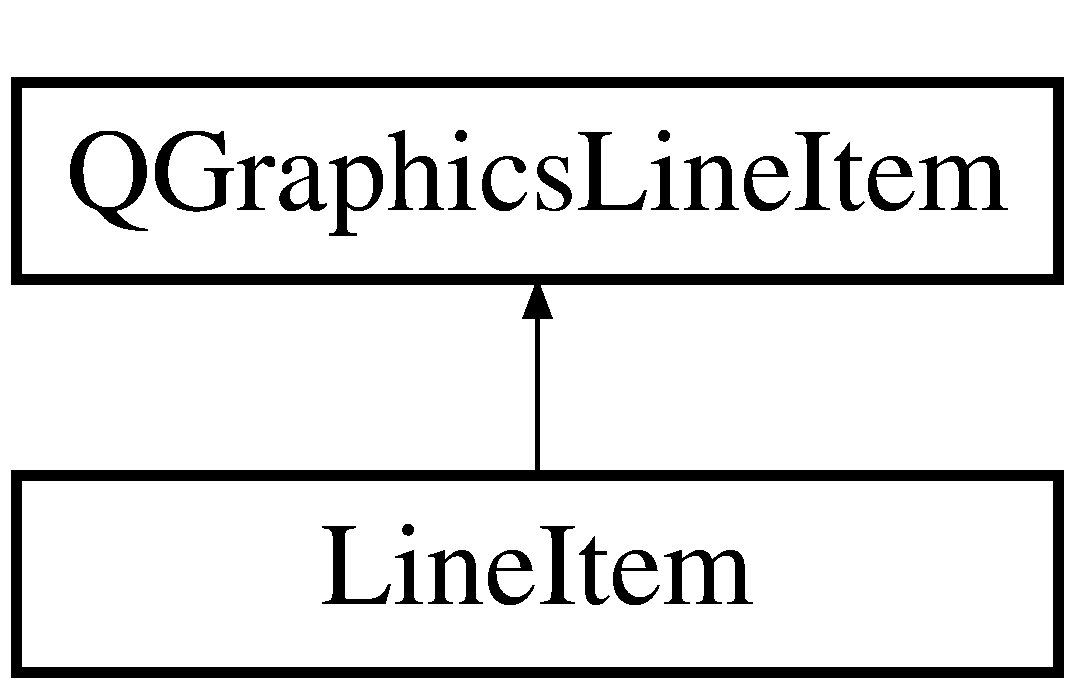
\includegraphics[height=2.000000cm]{classLineItem}
\end{center}
\end{figure}
\subsection*{Public Member Functions}
\begin{DoxyCompactItemize}
\item 
\mbox{\hyperlink{classLineItem_af79b99800cc44a69b53940bdb88ddd1b}{Line\+Item}} (unsigned x1, unsigned y1, unsigned x2, unsigned y2)
\begin{DoxyCompactList}\small\item\em Constructor for \mbox{\hyperlink{classLineItem}{Line\+Item}}. \end{DoxyCompactList}\item 
unsigned \mbox{\hyperlink{classLineItem_a8862ea60a3804d346e9801f79c67af76}{get\+X1}} ()
\begin{DoxyCompactList}\small\item\em Get start x coordinate. \end{DoxyCompactList}\item 
unsigned \mbox{\hyperlink{classLineItem_addce0ef5af72c233e2c7bf019c7a693d}{get\+X2}} ()
\begin{DoxyCompactList}\small\item\em Get end x coordinate. \end{DoxyCompactList}\item 
unsigned \mbox{\hyperlink{classLineItem_abbdf5be2637561802ea22385c7c11df5}{get\+Y1}} ()
\begin{DoxyCompactList}\small\item\em Get start y coordinate. \end{DoxyCompactList}\item 
unsigned \mbox{\hyperlink{classLineItem_aa99afab282d1e7e25b5d1549a41984d2}{get\+Y2}} ()
\begin{DoxyCompactList}\small\item\em Get end y coordinate. \end{DoxyCompactList}\item 
void \mbox{\hyperlink{classLineItem_acea090c7b9ff53dcc7a95ab7939b2cb9}{update\+Position}} (unsigned x\+\_\+new, unsigned y\+\_\+new)
\begin{DoxyCompactList}\small\item\em Update end x and y coordinates. \end{DoxyCompactList}\item 
bool \mbox{\hyperlink{classLineItem_af7dc675a032b27d6424536994095a95e}{is\+Inside}} (unsigned x, unsigned y)
\begin{DoxyCompactList}\small\item\em Check if coordinate is inside the item. \end{DoxyCompactList}\end{DoxyCompactItemize}
\subsection*{Static Public Attributes}
\begin{DoxyCompactItemize}
\item 
static const int \mbox{\hyperlink{classLineItem_af02da5c4e14746431c760eb075e3220e}{Compensation\+Value}} = 10
\item 
static Q\+Color \mbox{\hyperlink{classLineItem_a290f246bf61be323ebd52f68bfe9ab4d}{Line\+Color}} = Qt\+::black
\end{DoxyCompactItemize}


\subsection{Detailed Description}
Own implementation of Q\+Graphics\+Line\+Item. 

Adds coordinate positions variables to Q\+Graphics\+Line\+Item 

Definition at line 24 of file Line\+Item.\+hpp.



\subsection{Constructor \& Destructor Documentation}
\mbox{\Hypertarget{classLineItem_af79b99800cc44a69b53940bdb88ddd1b}\label{classLineItem_af79b99800cc44a69b53940bdb88ddd1b}} 
\index{Line\+Item@{Line\+Item}!Line\+Item@{Line\+Item}}
\index{Line\+Item@{Line\+Item}!Line\+Item@{Line\+Item}}
\subsubsection{\texorpdfstring{Line\+Item()}{LineItem()}}
{\footnotesize\ttfamily Line\+Item\+::\+Line\+Item (\begin{DoxyParamCaption}\item[{unsigned}]{x1,  }\item[{unsigned}]{y1,  }\item[{unsigned}]{x2,  }\item[{unsigned}]{y2 }\end{DoxyParamCaption})}



Constructor for \mbox{\hyperlink{classLineItem}{Line\+Item}}. 


\begin{DoxyParams}{Parameters}
{\em x1} & Start x coordinate \\
\hline
{\em y1} & Start y coordinate \\
\hline
{\em x2} & End x coordinate \\
\hline
{\em y2} & End y coordinate \\
\hline
\end{DoxyParams}


Definition at line 14 of file Line\+Item.\+cpp.



\subsection{Member Function Documentation}
\mbox{\Hypertarget{classLineItem_a8862ea60a3804d346e9801f79c67af76}\label{classLineItem_a8862ea60a3804d346e9801f79c67af76}} 
\index{Line\+Item@{Line\+Item}!get\+X1@{get\+X1}}
\index{get\+X1@{get\+X1}!Line\+Item@{Line\+Item}}
\subsubsection{\texorpdfstring{get\+X1()}{getX1()}}
{\footnotesize\ttfamily unsigned Line\+Item\+::get\+X1 (\begin{DoxyParamCaption}{ }\end{DoxyParamCaption})}



Get start x coordinate. 

\begin{DoxyReturn}{Returns}
Returns x1 
\end{DoxyReturn}


Definition at line 23 of file Line\+Item.\+cpp.

\mbox{\Hypertarget{classLineItem_addce0ef5af72c233e2c7bf019c7a693d}\label{classLineItem_addce0ef5af72c233e2c7bf019c7a693d}} 
\index{Line\+Item@{Line\+Item}!get\+X2@{get\+X2}}
\index{get\+X2@{get\+X2}!Line\+Item@{Line\+Item}}
\subsubsection{\texorpdfstring{get\+X2()}{getX2()}}
{\footnotesize\ttfamily unsigned Line\+Item\+::get\+X2 (\begin{DoxyParamCaption}{ }\end{DoxyParamCaption})}



Get end x coordinate. 

\begin{DoxyReturn}{Returns}
Returns x2 
\end{DoxyReturn}


Definition at line 28 of file Line\+Item.\+cpp.

\mbox{\Hypertarget{classLineItem_abbdf5be2637561802ea22385c7c11df5}\label{classLineItem_abbdf5be2637561802ea22385c7c11df5}} 
\index{Line\+Item@{Line\+Item}!get\+Y1@{get\+Y1}}
\index{get\+Y1@{get\+Y1}!Line\+Item@{Line\+Item}}
\subsubsection{\texorpdfstring{get\+Y1()}{getY1()}}
{\footnotesize\ttfamily unsigned Line\+Item\+::get\+Y1 (\begin{DoxyParamCaption}{ }\end{DoxyParamCaption})}



Get start y coordinate. 

\begin{DoxyReturn}{Returns}
Returns y1 
\end{DoxyReturn}


Definition at line 33 of file Line\+Item.\+cpp.

\mbox{\Hypertarget{classLineItem_aa99afab282d1e7e25b5d1549a41984d2}\label{classLineItem_aa99afab282d1e7e25b5d1549a41984d2}} 
\index{Line\+Item@{Line\+Item}!get\+Y2@{get\+Y2}}
\index{get\+Y2@{get\+Y2}!Line\+Item@{Line\+Item}}
\subsubsection{\texorpdfstring{get\+Y2()}{getY2()}}
{\footnotesize\ttfamily unsigned Line\+Item\+::get\+Y2 (\begin{DoxyParamCaption}{ }\end{DoxyParamCaption})}



Get end y coordinate. 

\begin{DoxyReturn}{Returns}
Returns y2 
\end{DoxyReturn}


Definition at line 38 of file Line\+Item.\+cpp.

\mbox{\Hypertarget{classLineItem_af7dc675a032b27d6424536994095a95e}\label{classLineItem_af7dc675a032b27d6424536994095a95e}} 
\index{Line\+Item@{Line\+Item}!is\+Inside@{is\+Inside}}
\index{is\+Inside@{is\+Inside}!Line\+Item@{Line\+Item}}
\subsubsection{\texorpdfstring{is\+Inside()}{isInside()}}
{\footnotesize\ttfamily bool Line\+Item\+::is\+Inside (\begin{DoxyParamCaption}\item[{unsigned}]{x,  }\item[{unsigned}]{y }\end{DoxyParamCaption})}



Check if coordinate is inside the item. 


\begin{DoxyParams}{Parameters}
{\em x} & x coordinate \\
\hline
{\em y} & y coordinate \\
\hline
\end{DoxyParams}
\begin{DoxyReturn}{Returns}
Returns true if the coordinate is inside the item 
\end{DoxyReturn}


Definition at line 51 of file Line\+Item.\+cpp.

\mbox{\Hypertarget{classLineItem_acea090c7b9ff53dcc7a95ab7939b2cb9}\label{classLineItem_acea090c7b9ff53dcc7a95ab7939b2cb9}} 
\index{Line\+Item@{Line\+Item}!update\+Position@{update\+Position}}
\index{update\+Position@{update\+Position}!Line\+Item@{Line\+Item}}
\subsubsection{\texorpdfstring{update\+Position()}{updatePosition()}}
{\footnotesize\ttfamily void Line\+Item\+::update\+Position (\begin{DoxyParamCaption}\item[{unsigned}]{x\+\_\+new,  }\item[{unsigned}]{y\+\_\+new }\end{DoxyParamCaption})}



Update end x and y coordinates. 


\begin{DoxyParams}{Parameters}
{\em x\+\_\+new} & New end x coordinate \\
\hline
{\em y\+\_\+new} & New end y coordinate \\
\hline
\end{DoxyParams}


Definition at line 43 of file Line\+Item.\+cpp.



\subsection{Member Data Documentation}
\mbox{\Hypertarget{classLineItem_af02da5c4e14746431c760eb075e3220e}\label{classLineItem_af02da5c4e14746431c760eb075e3220e}} 
\index{Line\+Item@{Line\+Item}!Compensation\+Value@{Compensation\+Value}}
\index{Compensation\+Value@{Compensation\+Value}!Line\+Item@{Line\+Item}}
\subsubsection{\texorpdfstring{Compensation\+Value}{CompensationValue}}
{\footnotesize\ttfamily const int Line\+Item\+::\+Compensation\+Value = 10\hspace{0.3cm}{\ttfamily [static]}}

Value used to compensate clicking the item to make it easier 

Definition at line 28 of file Line\+Item.\+hpp.

\mbox{\Hypertarget{classLineItem_a290f246bf61be323ebd52f68bfe9ab4d}\label{classLineItem_a290f246bf61be323ebd52f68bfe9ab4d}} 
\index{Line\+Item@{Line\+Item}!Line\+Color@{Line\+Color}}
\index{Line\+Color@{Line\+Color}!Line\+Item@{Line\+Item}}
\subsubsection{\texorpdfstring{Line\+Color}{LineColor}}
{\footnotesize\ttfamily Q\+Color Line\+Item\+::\+Line\+Color = Qt\+::black\hspace{0.3cm}{\ttfamily [static]}}

Color for Line\+Items, can be reset via \mbox{\hyperlink{classGUI}{G\+UI}} 

Definition at line 29 of file Line\+Item.\+hpp.



The documentation for this class was generated from the following files\+:\begin{DoxyCompactItemize}
\item 
include/\mbox{\hyperlink{LineItem_8hpp}{Line\+Item.\+hpp}}\item 
src/\mbox{\hyperlink{LineItem_8cpp}{Line\+Item.\+cpp}}\end{DoxyCompactItemize}

\hypertarget{classMainWidget}{}\section{Main\+Widget Class Reference}
\label{classMainWidget}\index{Main\+Widget@{Main\+Widget}}


{\ttfamily \#include $<$mainwidget.\+hpp$>$}

Inheritance diagram for Main\+Widget\+:\begin{figure}[H]
\begin{center}
\leavevmode
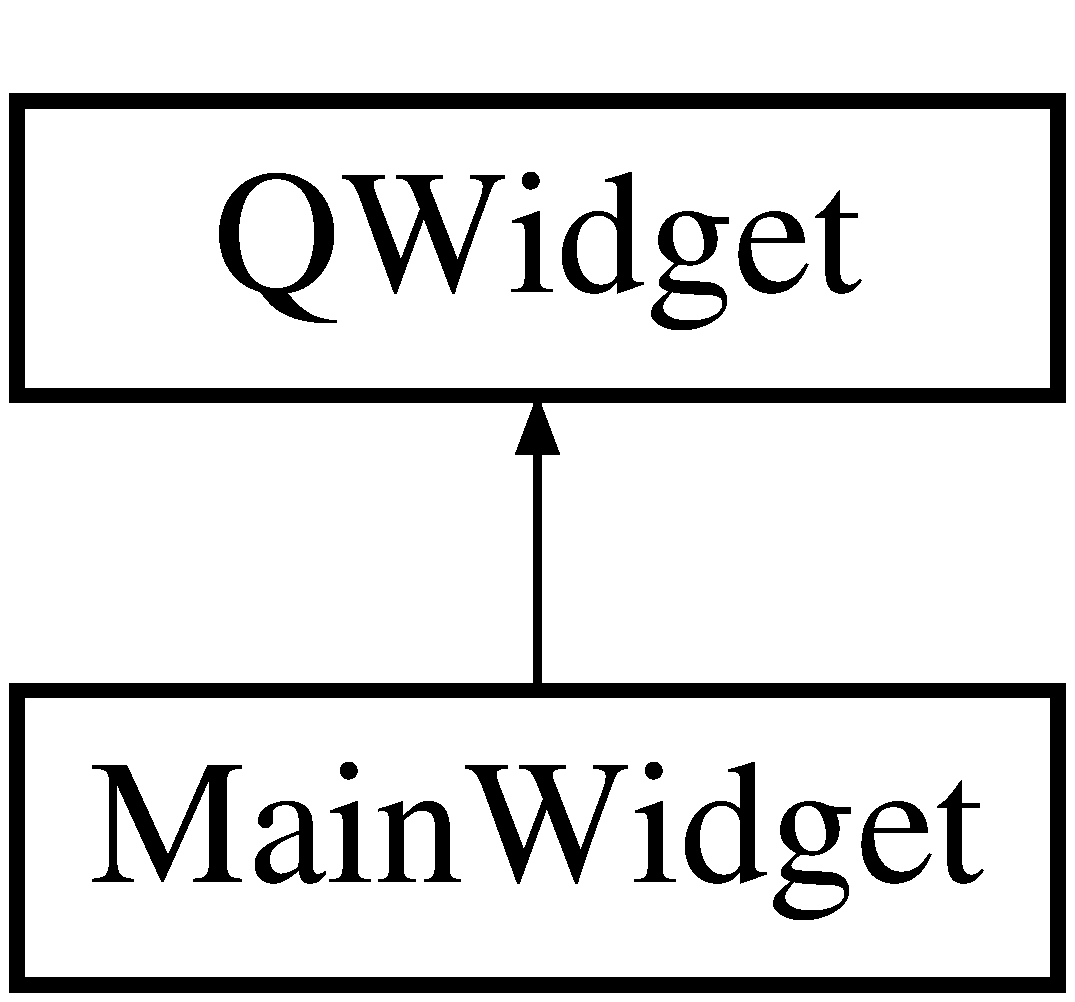
\includegraphics[height=2.000000cm]{classMainWidget}
\end{center}
\end{figure}
\subsection*{Public Member Functions}
\begin{DoxyCompactItemize}
\item 
\mbox{\hyperlink{classMainWidget_a62f5aa5fe2314c6221ac49b328b72e8b}{Main\+Widget}} (Q\+Widget $\ast$parent)
\begin{DoxyCompactList}\small\item\em Constructor for \mbox{\hyperlink{classMainWidget}{Main\+Widget}}. \end{DoxyCompactList}\item 
\mbox{\Hypertarget{classMainWidget_add21c63f8e799303a21a69da3d288c2f}\label{classMainWidget_add21c63f8e799303a21a69da3d288c2f}} 
\mbox{\hyperlink{classMainWidget_add21c63f8e799303a21a69da3d288c2f}{$\sim$\+Main\+Widget}} ()
\begin{DoxyCompactList}\small\item\em Deconstructor. \end{DoxyCompactList}\item 
\mbox{\hyperlink{classOwnGraphicsScene}{Own\+Graphics\+Scene}} $\ast$ \mbox{\hyperlink{classMainWidget_ad40a8bd13b501a0ebe88c87426a5b591}{get\+Scene}} ()
\begin{DoxyCompactList}\small\item\em Get the scene. \end{DoxyCompactList}\item 
Q\+Graphics\+View $\ast$ \mbox{\hyperlink{classMainWidget_ae73e3dac6fb1e99dabe84aab683b3fbd}{get\+View}} ()
\begin{DoxyCompactList}\small\item\em Get the view. \end{DoxyCompactList}\item 
Q\+H\+Box\+Layout $\ast$ \mbox{\hyperlink{classMainWidget_a639b465bb49eb31e1c09051ae047951f}{get\+Layout}} ()
\begin{DoxyCompactList}\small\item\em Get the layout. \end{DoxyCompactList}\item 
void \mbox{\hyperlink{classMainWidget_af544f3b04a81d63c0810a90706773d3d}{Init\+Scroll\+Bar}} ()
\begin{DoxyCompactList}\small\item\em Init the scrollbar. \end{DoxyCompactList}\end{DoxyCompactItemize}


\subsection{Detailed Description}
This class is the main widget for gui contains a Graphics scene and a view for it Uses Q\+H\+Box\+Layout 

Definition at line 34 of file mainwidget.\+hpp.



\subsection{Constructor \& Destructor Documentation}
\mbox{\Hypertarget{classMainWidget_a62f5aa5fe2314c6221ac49b328b72e8b}\label{classMainWidget_a62f5aa5fe2314c6221ac49b328b72e8b}} 
\index{Main\+Widget@{Main\+Widget}!Main\+Widget@{Main\+Widget}}
\index{Main\+Widget@{Main\+Widget}!Main\+Widget@{Main\+Widget}}
\subsubsection{\texorpdfstring{Main\+Widget()}{MainWidget()}}
{\footnotesize\ttfamily Main\+Widget\+::\+Main\+Widget (\begin{DoxyParamCaption}\item[{Q\+Widget $\ast$}]{parent }\end{DoxyParamCaption})}



Constructor for \mbox{\hyperlink{classMainWidget}{Main\+Widget}}. 


\begin{DoxyParams}{Parameters}
{\em parent} & the parent Q\+Widget \\
\hline
\end{DoxyParams}


Definition at line 13 of file mainwidget.\+cpp.



\subsection{Member Function Documentation}
\mbox{\Hypertarget{classMainWidget_a639b465bb49eb31e1c09051ae047951f}\label{classMainWidget_a639b465bb49eb31e1c09051ae047951f}} 
\index{Main\+Widget@{Main\+Widget}!get\+Layout@{get\+Layout}}
\index{get\+Layout@{get\+Layout}!Main\+Widget@{Main\+Widget}}
\subsubsection{\texorpdfstring{get\+Layout()}{getLayout()}}
{\footnotesize\ttfamily Q\+H\+Box\+Layout$\ast$ Main\+Widget\+::get\+Layout (\begin{DoxyParamCaption}{ }\end{DoxyParamCaption})\hspace{0.3cm}{\ttfamily [inline]}}



Get the layout. 

\begin{DoxyReturn}{Returns}
Returns the graphics layout 
\end{DoxyReturn}


Definition at line 67 of file mainwidget.\+hpp.

\mbox{\Hypertarget{classMainWidget_ad40a8bd13b501a0ebe88c87426a5b591}\label{classMainWidget_ad40a8bd13b501a0ebe88c87426a5b591}} 
\index{Main\+Widget@{Main\+Widget}!get\+Scene@{get\+Scene}}
\index{get\+Scene@{get\+Scene}!Main\+Widget@{Main\+Widget}}
\subsubsection{\texorpdfstring{get\+Scene()}{getScene()}}
{\footnotesize\ttfamily \mbox{\hyperlink{classOwnGraphicsScene}{Own\+Graphics\+Scene}}$\ast$ Main\+Widget\+::get\+Scene (\begin{DoxyParamCaption}{ }\end{DoxyParamCaption})\hspace{0.3cm}{\ttfamily [inline]}}



Get the scene. 

\begin{DoxyReturn}{Returns}
Returns the graphics scene 
\end{DoxyReturn}


Definition at line 57 of file mainwidget.\+hpp.

\mbox{\Hypertarget{classMainWidget_ae73e3dac6fb1e99dabe84aab683b3fbd}\label{classMainWidget_ae73e3dac6fb1e99dabe84aab683b3fbd}} 
\index{Main\+Widget@{Main\+Widget}!get\+View@{get\+View}}
\index{get\+View@{get\+View}!Main\+Widget@{Main\+Widget}}
\subsubsection{\texorpdfstring{get\+View()}{getView()}}
{\footnotesize\ttfamily Q\+Graphics\+View$\ast$ Main\+Widget\+::get\+View (\begin{DoxyParamCaption}{ }\end{DoxyParamCaption})\hspace{0.3cm}{\ttfamily [inline]}}



Get the view. 

\begin{DoxyReturn}{Returns}
Returns the graphics view 
\end{DoxyReturn}


Definition at line 62 of file mainwidget.\+hpp.

\mbox{\Hypertarget{classMainWidget_af544f3b04a81d63c0810a90706773d3d}\label{classMainWidget_af544f3b04a81d63c0810a90706773d3d}} 
\index{Main\+Widget@{Main\+Widget}!Init\+Scroll\+Bar@{Init\+Scroll\+Bar}}
\index{Init\+Scroll\+Bar@{Init\+Scroll\+Bar}!Main\+Widget@{Main\+Widget}}
\subsubsection{\texorpdfstring{Init\+Scroll\+Bar()}{InitScrollBar()}}
{\footnotesize\ttfamily void Main\+Widget\+::\+Init\+Scroll\+Bar (\begin{DoxyParamCaption}{ }\end{DoxyParamCaption})}



Init the scrollbar. 

Set view scrollbar to left and center of the scene 

Definition at line 37 of file mainwidget.\+cpp.



The documentation for this class was generated from the following files\+:\begin{DoxyCompactItemize}
\item 
include/\mbox{\hyperlink{mainwidget_8hpp}{mainwidget.\+hpp}}\item 
src/\mbox{\hyperlink{mainwidget_8cpp}{mainwidget.\+cpp}}\end{DoxyCompactItemize}

\hypertarget{structModeToolbar}{}\section{Mode\+Toolbar Struct Reference}
\label{structModeToolbar}\index{Mode\+Toolbar@{Mode\+Toolbar}}


Toolbar for changing image cut mode.  




{\ttfamily \#include $<$gui.\+hpp$>$}

\subsection*{Public Attributes}
\begin{DoxyCompactItemize}
\item 
Q\+Tool\+Bar $\ast$ \mbox{\hyperlink{structModeToolbar_acc6bcdd91825343f34ec38d312418234}{mode\+\_\+toolbar}}
\item 
Q\+Combo\+Box $\ast$ \mbox{\hyperlink{structModeToolbar_ad0ba4f03ef2a44e2543add404a50b4f1}{combobox}}
\item 
Q\+Action $\ast$ \mbox{\hyperlink{structModeToolbar_af7d7766f5b1710abb382c42689e963ca}{continue\+\_\+button}}
\item 
Q\+Action $\ast$ \mbox{\hyperlink{structModeToolbar_a814fa4aec4ff40543904dfc4aa4c8e89}{cancel}}
\end{DoxyCompactItemize}


\subsection{Detailed Description}
Toolbar for changing image cut mode. 

Definition at line 129 of file gui.\+hpp.



\subsection{Member Data Documentation}
\mbox{\Hypertarget{structModeToolbar_a814fa4aec4ff40543904dfc4aa4c8e89}\label{structModeToolbar_a814fa4aec4ff40543904dfc4aa4c8e89}} 
\index{Mode\+Toolbar@{Mode\+Toolbar}!cancel@{cancel}}
\index{cancel@{cancel}!Mode\+Toolbar@{Mode\+Toolbar}}
\subsubsection{\texorpdfstring{cancel}{cancel}}
{\footnotesize\ttfamily Q\+Action$\ast$ Mode\+Toolbar\+::cancel}

Pointer to a Q\+Action which connects to Cancel\+From\+Mode 

Definition at line 134 of file gui.\+hpp.

\mbox{\Hypertarget{structModeToolbar_ad0ba4f03ef2a44e2543add404a50b4f1}\label{structModeToolbar_ad0ba4f03ef2a44e2543add404a50b4f1}} 
\index{Mode\+Toolbar@{Mode\+Toolbar}!combobox@{combobox}}
\index{combobox@{combobox}!Mode\+Toolbar@{Mode\+Toolbar}}
\subsubsection{\texorpdfstring{combobox}{combobox}}
{\footnotesize\ttfamily Q\+Combo\+Box$\ast$ Mode\+Toolbar\+::combobox}

Pointer to the Q\+Combo\+Box 

Definition at line 132 of file gui.\+hpp.

\mbox{\Hypertarget{structModeToolbar_af7d7766f5b1710abb382c42689e963ca}\label{structModeToolbar_af7d7766f5b1710abb382c42689e963ca}} 
\index{Mode\+Toolbar@{Mode\+Toolbar}!continue\+\_\+button@{continue\+\_\+button}}
\index{continue\+\_\+button@{continue\+\_\+button}!Mode\+Toolbar@{Mode\+Toolbar}}
\subsubsection{\texorpdfstring{continue\+\_\+button}{continue\_button}}
{\footnotesize\ttfamily Q\+Action$\ast$ Mode\+Toolbar\+::continue\+\_\+button}

Pointer to a Q\+Action which connects to Continue\+From\+Mode 

Definition at line 133 of file gui.\+hpp.

\mbox{\Hypertarget{structModeToolbar_acc6bcdd91825343f34ec38d312418234}\label{structModeToolbar_acc6bcdd91825343f34ec38d312418234}} 
\index{Mode\+Toolbar@{Mode\+Toolbar}!mode\+\_\+toolbar@{mode\+\_\+toolbar}}
\index{mode\+\_\+toolbar@{mode\+\_\+toolbar}!Mode\+Toolbar@{Mode\+Toolbar}}
\subsubsection{\texorpdfstring{mode\+\_\+toolbar}{mode\_toolbar}}
{\footnotesize\ttfamily Q\+Tool\+Bar$\ast$ Mode\+Toolbar\+::mode\+\_\+toolbar}

Pointer to the Q\+Toolbar 

Definition at line 131 of file gui.\+hpp.



The documentation for this struct was generated from the following file\+:\begin{DoxyCompactItemize}
\item 
include/\mbox{\hyperlink{gui_8hpp}{gui.\+hpp}}\end{DoxyCompactItemize}

\hypertarget{classOwnGraphicsScene}{}\section{Own\+Graphics\+Scene Class Reference}
\label{classOwnGraphicsScene}\index{Own\+Graphics\+Scene@{Own\+Graphics\+Scene}}
Inheritance diagram for Own\+Graphics\+Scene\+:\begin{figure}[H]
\begin{center}
\leavevmode
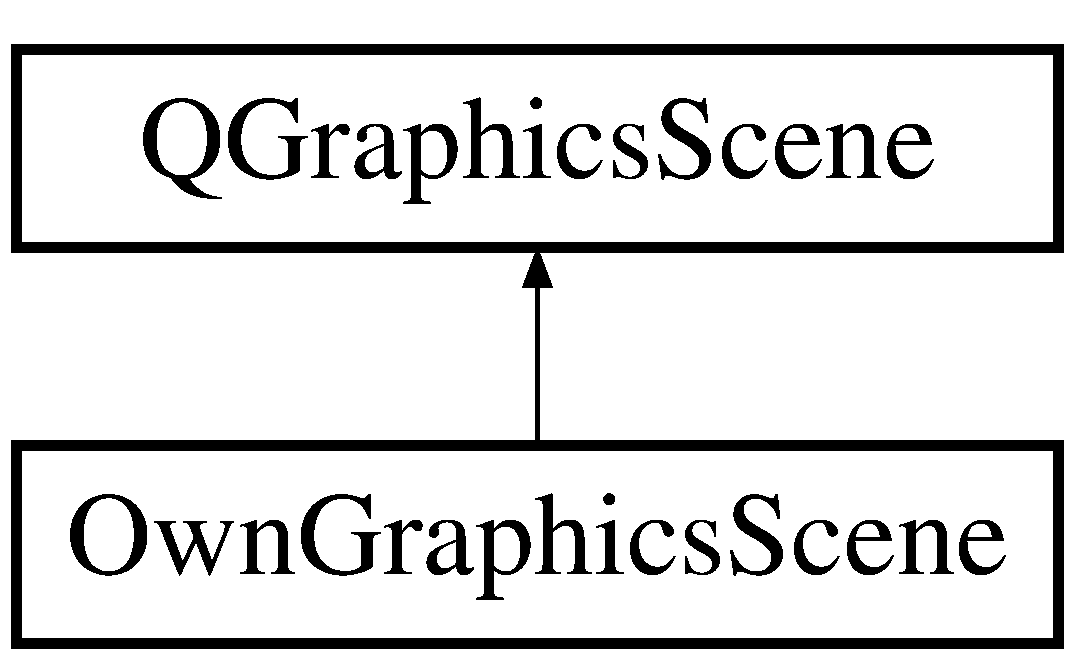
\includegraphics[height=2.000000cm]{classOwnGraphicsScene}
\end{center}
\end{figure}
\subsection*{Public Member Functions}
\begin{DoxyCompactItemize}
\item 
\mbox{\Hypertarget{classOwnGraphicsScene_a242b82147a469314e4c7fb5af69c265f}\label{classOwnGraphicsScene_a242b82147a469314e4c7fb5af69c265f}} 
{\bfseries Own\+Graphics\+Scene} (Q\+Widget $\ast$parent)
\item 
\mbox{\Hypertarget{classOwnGraphicsScene_a1a9916971af608d5331483606f72fbe4}\label{classOwnGraphicsScene_a1a9916971af608d5331483606f72fbe4}} 
void {\bfseries mouse\+Press\+Event} (Q\+Graphics\+Scene\+Mouse\+Event $\ast$event)
\item 
\mbox{\Hypertarget{classOwnGraphicsScene_ac7f6be2800f09463413459fed74bf34e}\label{classOwnGraphicsScene_ac7f6be2800f09463413459fed74bf34e}} 
void {\bfseries mouse\+Move\+Event} (Q\+Graphics\+Scene\+Mouse\+Event $\ast$event)
\item 
\mbox{\Hypertarget{classOwnGraphicsScene_a4251b836ee575083f4eeaa73254723f4}\label{classOwnGraphicsScene_a4251b836ee575083f4eeaa73254723f4}} 
\mbox{\hyperlink{classLineItem}{Line\+Item}} $\ast$ {\bfseries add\+Line} (unsigned x1, unsigned y1, unsigned x2, unsigned y2)
\item 
\mbox{\Hypertarget{classOwnGraphicsScene_a6e54bd43db758bcd4f7cc1dd4544232e}\label{classOwnGraphicsScene_a6e54bd43db758bcd4f7cc1dd4544232e}} 
unsigned {\bfseries get\+MouseX} ()
\item 
\mbox{\Hypertarget{classOwnGraphicsScene_a3fd2942e9930fc2dda41844622dc8a35}\label{classOwnGraphicsScene_a3fd2942e9930fc2dda41844622dc8a35}} 
unsigned {\bfseries get\+MouseY} ()
\item 
\mbox{\Hypertarget{classOwnGraphicsScene_a6b7e69131827f0ae64626af378ff9974}\label{classOwnGraphicsScene_a6b7e69131827f0ae64626af378ff9974}} 
void {\bfseries Line\+Mode} (bool activate)
\item 
\mbox{\Hypertarget{classOwnGraphicsScene_aca454942ecf6c472d020e063862464d4}\label{classOwnGraphicsScene_aca454942ecf6c472d020e063862464d4}} 
void {\bfseries Delete\+Mode} (bool activate)
\item 
\mbox{\Hypertarget{classOwnGraphicsScene_a31221ca321dde1e684f9cdf23dd1c225}\label{classOwnGraphicsScene_a31221ca321dde1e684f9cdf23dd1c225}} 
void {\bfseries Clear\+Mode} ()
\item 
\mbox{\Hypertarget{classOwnGraphicsScene_a5b4b466a697f83c23294a80067edac23}\label{classOwnGraphicsScene_a5b4b466a697f83c23294a80067edac23}} 
void {\bfseries remove\+\_\+\+Item} (unsigned x, unsigned y)
\item 
\mbox{\Hypertarget{classOwnGraphicsScene_a8d133a1b72a853772d2d89da4d4e1afa}\label{classOwnGraphicsScene_a8d133a1b72a853772d2d89da4d4e1afa}} 
void {\bfseries Clear\+All} ()
\item 
\mbox{\Hypertarget{classOwnGraphicsScene_ae83ee24e342b50c335af155a34295185}\label{classOwnGraphicsScene_ae83ee24e342b50c335af155a34295185}} 
bool {\bfseries set\+Image} (Q\+String imagename)
\item 
\mbox{\Hypertarget{classOwnGraphicsScene_acc6e7978a3f10889e439ceabd155a341}\label{classOwnGraphicsScene_acc6e7978a3f10889e439ceabd155a341}} 
bool {\bfseries img\+Mode} (bool activate)
\item 
\mbox{\Hypertarget{classOwnGraphicsScene_aefe52a5b20dbb38dcc9d9510ecfabe52}\label{classOwnGraphicsScene_aefe52a5b20dbb38dcc9d9510ecfabe52}} 
void {\bfseries Delete\+Img\+Mode} (bool activate)
\item 
\mbox{\Hypertarget{classOwnGraphicsScene_abda962c04f88920377d3bb23b30b9267}\label{classOwnGraphicsScene_abda962c04f88920377d3bb23b30b9267}} 
void {\bfseries Delete\+Img} (unsigned x1, unsigned y1)
\item 
\mbox{\Hypertarget{classOwnGraphicsScene_a3ce5a34cebcc134ecb20323c48e5812b}\label{classOwnGraphicsScene_a3ce5a34cebcc134ecb20323c48e5812b}} 
void {\bfseries Cut\+Image\+Mode} (bool active)
\item 
\mbox{\Hypertarget{classOwnGraphicsScene_ae79aa179ce90ab26f06d7d17eed96b93}\label{classOwnGraphicsScene_ae79aa179ce90ab26f06d7d17eed96b93}} 
bool {\bfseries Select\+Cut\+Img} ()
\item 
\mbox{\Hypertarget{classOwnGraphicsScene_a656919c9fdd0827ae182d3d3f5f91e4f}\label{classOwnGraphicsScene_a656919c9fdd0827ae182d3d3f5f91e4f}} 
void {\bfseries Set\+Img\+Cut\+Mode} (int cut\+\_\+mode)
\item 
\mbox{\Hypertarget{classOwnGraphicsScene_a7e3d97c27cca1df796b75cc4a99e24cd}\label{classOwnGraphicsScene_a7e3d97c27cca1df796b75cc4a99e24cd}} 
void {\bfseries Cut\+Pixmap\+Item} ()
\item 
\mbox{\Hypertarget{classOwnGraphicsScene_a4976a8e6f682612acd3e23b6c98bd8d8}\label{classOwnGraphicsScene_a4976a8e6f682612acd3e23b6c98bd8d8}} 
void {\bfseries Remove\+Poly\+Previous} ()
\item 
\mbox{\Hypertarget{classOwnGraphicsScene_ad62254e1884fa4817ff1beaa3bc6c011}\label{classOwnGraphicsScene_ad62254e1884fa4817ff1beaa3bc6c011}} 
void {\bfseries set\+Connect\+Lines} (int value)
\item 
\mbox{\Hypertarget{classOwnGraphicsScene_a158c6430ca8e07642b693e37ec05119e}\label{classOwnGraphicsScene_a158c6430ca8e07642b693e37ec05119e}} 
void {\bfseries Clear\+Visual\+Items} ()
\end{DoxyCompactItemize}


\subsection{Detailed Description}


Definition at line 70 of file owngraphicsscene.\+hpp.



The documentation for this class was generated from the following files\+:\begin{DoxyCompactItemize}
\item 
include/owngraphicsscene.\+hpp\item 
src/owngraphicsscene.\+cpp\end{DoxyCompactItemize}

\hypertarget{classPixmapItem}{}\section{Pixmap\+Item Class Reference}
\label{classPixmapItem}\index{Pixmap\+Item@{Pixmap\+Item}}


Own Q\+Graphics\+Pixmap\+Item implementation.  




{\ttfamily \#include $<$Pixmap\+Item.\+hpp$>$}

Inheritance diagram for Pixmap\+Item\+:\begin{figure}[H]
\begin{center}
\leavevmode
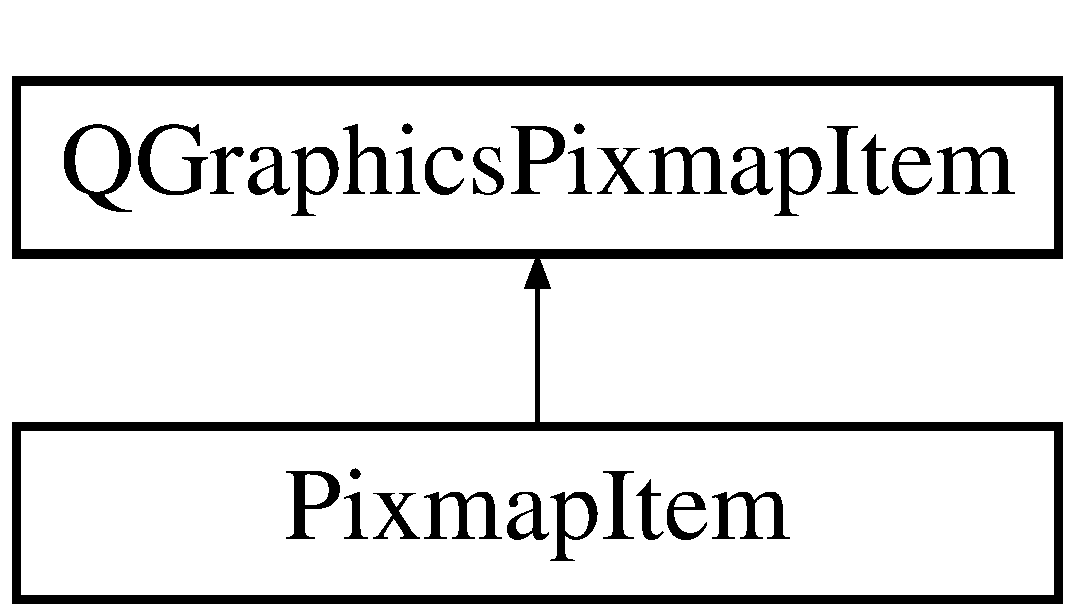
\includegraphics[height=2.000000cm]{classPixmapItem}
\end{center}
\end{figure}
\subsection*{Public Member Functions}
\begin{DoxyCompactItemize}
\item 
\mbox{\hyperlink{classPixmapItem_a7e339e581be3c4892d2af89494bd137c}{Pixmap\+Item}} (Q\+Pixmap pixmap, Q\+String image\+\_\+name)
\begin{DoxyCompactList}\small\item\em Constructor for \mbox{\hyperlink{classPixmapItem}{Pixmap\+Item}}. \end{DoxyCompactList}\item 
bool \mbox{\hyperlink{classPixmapItem_ad5510bf5a97b352e3b06cb888ac0a99c}{is\+Xinside}} (unsigned x)
\begin{DoxyCompactList}\small\item\em Is x coordinate inside the item. \end{DoxyCompactList}\item 
bool \mbox{\hyperlink{classPixmapItem_ab6e6526fd5cd0ce5ba34b665adca6c5c}{is\+Yinside}} (unsigned y)
\begin{DoxyCompactList}\small\item\em Is y coordinate inside the item. \end{DoxyCompactList}\item 
void \mbox{\hyperlink{classPixmapItem_a692a0aca72ffbe102769fdc9246ed2f6}{setX}} (unsigned x)
\begin{DoxyCompactList}\small\item\em Set new x coordinate. \end{DoxyCompactList}\item 
void \mbox{\hyperlink{classPixmapItem_a6c6f4a872823f585edcf134d9bf209e1}{setY}} (unsigned y)
\begin{DoxyCompactList}\small\item\em Set new y coordinate. \end{DoxyCompactList}\item 
void \mbox{\hyperlink{classPixmapItem_a6e18b1223f61d40dba6e96f4da15ce5c}{add\+Painter\+Point}} (unsigned x, unsigned y)
\begin{DoxyCompactList}\small\item\em Add Q\+Point to painter\+\_\+points. \end{DoxyCompactList}\item 
void \mbox{\hyperlink{classPixmapItem_a54810877049ab858d569f83065720a18}{clear\+Points\+Vector}} ()
\begin{DoxyCompactList}\small\item\em Clear all Q\+Points of the item. \end{DoxyCompactList}\item 
void \mbox{\hyperlink{classPixmapItem_a4a742318dce01d018da2f4b01790c210}{Cut\+Item}} ()
\begin{DoxyCompactList}\small\item\em Cut the item. \end{DoxyCompactList}\item 
void \mbox{\hyperlink{classPixmapItem_ae2e67a7b69ef10dc613e14c1d3c1a327}{Remove\+Latest\+Point}} ()
\begin{DoxyCompactList}\small\item\em Remove the latest point added. \end{DoxyCompactList}\item 
void \mbox{\hyperlink{classPixmapItem_ab71710e3b66024a62fe56a43e60141b3}{Line\+Cut}} ()
\begin{DoxyCompactList}\small\item\em Cut item based on a \mbox{\hyperlink{classLineItem}{Line\+Item}}. \end{DoxyCompactList}\item 
void \mbox{\hyperlink{classPixmapItem_a660c7d73c4f915e6673a3b602affb568}{Bezier\+Cut}} ()
\begin{DoxyCompactList}\small\item\em Cut item based on a \mbox{\hyperlink{classBezier}{Bezier}} (its Line\+Items) \end{DoxyCompactList}\end{DoxyCompactItemize}
\subsection*{Static Public Attributes}
\begin{DoxyCompactItemize}
\item 
static \mbox{\hyperlink{namespaceEditor_aad9ecf07f59416285836e79f1b1d2bd8}{Editor\+::\+Connect\+Point}} \mbox{\hyperlink{classPixmapItem_a3733ea98fc45c24acc1bc1552e969895}{connect\+\_\+point}} = Editor\+::\+Connect\+Point\+::\+Connect\+Zero
\end{DoxyCompactItemize}


\subsection{Detailed Description}
Own Q\+Graphics\+Pixmap\+Item implementation. 

This class inherits Q\+Graphics\+Pixmap\+Item Adds a position specifiers to the base class 

Definition at line 60 of file Pixmap\+Item.\+hpp.



\subsection{Constructor \& Destructor Documentation}
\mbox{\Hypertarget{classPixmapItem_a7e339e581be3c4892d2af89494bd137c}\label{classPixmapItem_a7e339e581be3c4892d2af89494bd137c}} 
\index{Pixmap\+Item@{Pixmap\+Item}!Pixmap\+Item@{Pixmap\+Item}}
\index{Pixmap\+Item@{Pixmap\+Item}!Pixmap\+Item@{Pixmap\+Item}}
\subsubsection{\texorpdfstring{Pixmap\+Item()}{PixmapItem()}}
{\footnotesize\ttfamily Pixmap\+Item\+::\+Pixmap\+Item (\begin{DoxyParamCaption}\item[{Q\+Pixmap}]{pixmap,  }\item[{Q\+String}]{image\+\_\+name }\end{DoxyParamCaption})}



Constructor for \mbox{\hyperlink{classPixmapItem}{Pixmap\+Item}}. 


\begin{DoxyParams}{Parameters}
{\em pixmap} & Pixmap which the item is created from \\
\hline
{\em image\+\_\+name} & Name(path) of the image used in Pixmap \\
\hline
\end{DoxyParams}


Definition at line 19 of file Pixmap\+Item.\+cpp.



\subsection{Member Function Documentation}
\mbox{\Hypertarget{classPixmapItem_a6e18b1223f61d40dba6e96f4da15ce5c}\label{classPixmapItem_a6e18b1223f61d40dba6e96f4da15ce5c}} 
\index{Pixmap\+Item@{Pixmap\+Item}!add\+Painter\+Point@{add\+Painter\+Point}}
\index{add\+Painter\+Point@{add\+Painter\+Point}!Pixmap\+Item@{Pixmap\+Item}}
\subsubsection{\texorpdfstring{add\+Painter\+Point()}{addPainterPoint()}}
{\footnotesize\ttfamily void Pixmap\+Item\+::add\+Painter\+Point (\begin{DoxyParamCaption}\item[{unsigned}]{x,  }\item[{unsigned}]{y }\end{DoxyParamCaption})}



Add Q\+Point to painter\+\_\+points. 


\begin{DoxyParams}{Parameters}
{\em x} & x coordinate of the point \\
\hline
{\em y} & y coordinate of the point\\
\hline
\end{DoxyParams}
The painter point is used in cut image mode to create a polygon cut 

Definition at line 102 of file Pixmap\+Item.\+cpp.

\mbox{\Hypertarget{classPixmapItem_a660c7d73c4f915e6673a3b602affb568}\label{classPixmapItem_a660c7d73c4f915e6673a3b602affb568}} 
\index{Pixmap\+Item@{Pixmap\+Item}!Bezier\+Cut@{Bezier\+Cut}}
\index{Bezier\+Cut@{Bezier\+Cut}!Pixmap\+Item@{Pixmap\+Item}}
\subsubsection{\texorpdfstring{Bezier\+Cut()}{BezierCut()}}
{\footnotesize\ttfamily void Pixmap\+Item\+::\+Bezier\+Cut (\begin{DoxyParamCaption}{ }\end{DoxyParamCaption})}



Cut item based on a \mbox{\hyperlink{classBezier}{Bezier}} (its Line\+Items) 

Connects lines from the last painter\+\_\+point to the first using lower edge as a connection point 

Definition at line 172 of file Pixmap\+Item.\+cpp.

\mbox{\Hypertarget{classPixmapItem_a54810877049ab858d569f83065720a18}\label{classPixmapItem_a54810877049ab858d569f83065720a18}} 
\index{Pixmap\+Item@{Pixmap\+Item}!clear\+Points\+Vector@{clear\+Points\+Vector}}
\index{clear\+Points\+Vector@{clear\+Points\+Vector}!Pixmap\+Item@{Pixmap\+Item}}
\subsubsection{\texorpdfstring{clear\+Points\+Vector()}{clearPointsVector()}}
{\footnotesize\ttfamily void Pixmap\+Item\+::clear\+Points\+Vector (\begin{DoxyParamCaption}{ }\end{DoxyParamCaption})}



Clear all Q\+Points of the item. 

Points are cleared from painter\+\_\+points vector 

Definition at line 116 of file Pixmap\+Item.\+cpp.

\mbox{\Hypertarget{classPixmapItem_a4a742318dce01d018da2f4b01790c210}\label{classPixmapItem_a4a742318dce01d018da2f4b01790c210}} 
\index{Pixmap\+Item@{Pixmap\+Item}!Cut\+Item@{Cut\+Item}}
\index{Cut\+Item@{Cut\+Item}!Pixmap\+Item@{Pixmap\+Item}}
\subsubsection{\texorpdfstring{Cut\+Item()}{CutItem()}}
{\footnotesize\ttfamily void Pixmap\+Item\+::\+Cut\+Item (\begin{DoxyParamCaption}{ }\end{DoxyParamCaption})}



Cut the item. 

Cut path is defined by Q\+Painter\+Path which is created from Q\+Points in painter\+\_\+points 

Definition at line 33 of file Pixmap\+Item.\+cpp.

\mbox{\Hypertarget{classPixmapItem_ad5510bf5a97b352e3b06cb888ac0a99c}\label{classPixmapItem_ad5510bf5a97b352e3b06cb888ac0a99c}} 
\index{Pixmap\+Item@{Pixmap\+Item}!is\+Xinside@{is\+Xinside}}
\index{is\+Xinside@{is\+Xinside}!Pixmap\+Item@{Pixmap\+Item}}
\subsubsection{\texorpdfstring{is\+Xinside()}{isXinside()}}
{\footnotesize\ttfamily bool Pixmap\+Item\+::is\+Xinside (\begin{DoxyParamCaption}\item[{unsigned}]{x }\end{DoxyParamCaption})}



Is x coordinate inside the item. 


\begin{DoxyParams}{Parameters}
{\em x} & x coordinate \\
\hline
\end{DoxyParams}
\begin{DoxyReturn}{Returns}
Returns true if x is inside the item 
\end{DoxyReturn}


Definition at line 68 of file Pixmap\+Item.\+cpp.

\mbox{\Hypertarget{classPixmapItem_ab6e6526fd5cd0ce5ba34b665adca6c5c}\label{classPixmapItem_ab6e6526fd5cd0ce5ba34b665adca6c5c}} 
\index{Pixmap\+Item@{Pixmap\+Item}!is\+Yinside@{is\+Yinside}}
\index{is\+Yinside@{is\+Yinside}!Pixmap\+Item@{Pixmap\+Item}}
\subsubsection{\texorpdfstring{is\+Yinside()}{isYinside()}}
{\footnotesize\ttfamily bool Pixmap\+Item\+::is\+Yinside (\begin{DoxyParamCaption}\item[{unsigned}]{y }\end{DoxyParamCaption})}



Is y coordinate inside the item. 


\begin{DoxyParams}{Parameters}
{\em y} & y coordinate \\
\hline
\end{DoxyParams}
\begin{DoxyReturn}{Returns}
Returns true if y is inside the item 
\end{DoxyReturn}


Definition at line 80 of file Pixmap\+Item.\+cpp.

\mbox{\Hypertarget{classPixmapItem_ab71710e3b66024a62fe56a43e60141b3}\label{classPixmapItem_ab71710e3b66024a62fe56a43e60141b3}} 
\index{Pixmap\+Item@{Pixmap\+Item}!Line\+Cut@{Line\+Cut}}
\index{Line\+Cut@{Line\+Cut}!Pixmap\+Item@{Pixmap\+Item}}
\subsubsection{\texorpdfstring{Line\+Cut()}{LineCut()}}
{\footnotesize\ttfamily void Pixmap\+Item\+::\+Line\+Cut (\begin{DoxyParamCaption}{ }\end{DoxyParamCaption})}



Cut item based on a \mbox{\hyperlink{classLineItem}{Line\+Item}}. 

Connects lines from lower edges of the pixmap to the \mbox{\hyperlink{classLineItem}{Line\+Item}} points 

Definition at line 136 of file Pixmap\+Item.\+cpp.

\mbox{\Hypertarget{classPixmapItem_ae2e67a7b69ef10dc613e14c1d3c1a327}\label{classPixmapItem_ae2e67a7b69ef10dc613e14c1d3c1a327}} 
\index{Pixmap\+Item@{Pixmap\+Item}!Remove\+Latest\+Point@{Remove\+Latest\+Point}}
\index{Remove\+Latest\+Point@{Remove\+Latest\+Point}!Pixmap\+Item@{Pixmap\+Item}}
\subsubsection{\texorpdfstring{Remove\+Latest\+Point()}{RemoveLatestPoint()}}
{\footnotesize\ttfamily void Pixmap\+Item\+::\+Remove\+Latest\+Point (\begin{DoxyParamCaption}{ }\end{DoxyParamCaption})}



Remove the latest point added. 

Removes the latest entry from painter\+\_\+points vector 

Definition at line 126 of file Pixmap\+Item.\+cpp.

\mbox{\Hypertarget{classPixmapItem_a692a0aca72ffbe102769fdc9246ed2f6}\label{classPixmapItem_a692a0aca72ffbe102769fdc9246ed2f6}} 
\index{Pixmap\+Item@{Pixmap\+Item}!setX@{setX}}
\index{setX@{setX}!Pixmap\+Item@{Pixmap\+Item}}
\subsubsection{\texorpdfstring{set\+X()}{setX()}}
{\footnotesize\ttfamily void Pixmap\+Item\+::setX (\begin{DoxyParamCaption}\item[{unsigned}]{x }\end{DoxyParamCaption})}



Set new x coordinate. 


\begin{DoxyParams}{Parameters}
{\em x} & New x coordinate \\
\hline
\end{DoxyParams}


Definition at line 89 of file Pixmap\+Item.\+cpp.

\mbox{\Hypertarget{classPixmapItem_a6c6f4a872823f585edcf134d9bf209e1}\label{classPixmapItem_a6c6f4a872823f585edcf134d9bf209e1}} 
\index{Pixmap\+Item@{Pixmap\+Item}!setY@{setY}}
\index{setY@{setY}!Pixmap\+Item@{Pixmap\+Item}}
\subsubsection{\texorpdfstring{set\+Y()}{setY()}}
{\footnotesize\ttfamily void Pixmap\+Item\+::setY (\begin{DoxyParamCaption}\item[{unsigned}]{y }\end{DoxyParamCaption})}



Set new y coordinate. 


\begin{DoxyParams}{Parameters}
{\em y} & New y coordinate \\
\hline
\end{DoxyParams}


Definition at line 94 of file Pixmap\+Item.\+cpp.



\subsection{Member Data Documentation}
\mbox{\Hypertarget{classPixmapItem_a3733ea98fc45c24acc1bc1552e969895}\label{classPixmapItem_a3733ea98fc45c24acc1bc1552e969895}} 
\index{Pixmap\+Item@{Pixmap\+Item}!connect\+\_\+point@{connect\+\_\+point}}
\index{connect\+\_\+point@{connect\+\_\+point}!Pixmap\+Item@{Pixmap\+Item}}
\subsubsection{\texorpdfstring{connect\+\_\+point}{connect\_point}}
{\footnotesize\ttfamily \mbox{\hyperlink{namespaceEditor_aad9ecf07f59416285836e79f1b1d2bd8}{Editor\+::\+Connect\+Point}} Pixmap\+Item\+::connect\+\_\+point = Editor\+::\+Connect\+Point\+::\+Connect\+Zero\hspace{0.3cm}{\ttfamily [static]}}

Tells to which point Line\+Cut and Bezier\+Cut connect cut paths in y dimension. 

Definition at line 63 of file Pixmap\+Item.\+hpp.



The documentation for this class was generated from the following files\+:\begin{DoxyCompactItemize}
\item 
include/\mbox{\hyperlink{PixmapItem_8hpp}{Pixmap\+Item.\+hpp}}\item 
src/\mbox{\hyperlink{PixmapItem_8cpp}{Pixmap\+Item.\+cpp}}\end{DoxyCompactItemize}

\hypertarget{structPolygonToolbar}{}\section{Polygon\+Toolbar Struct Reference}
\label{structPolygonToolbar}\index{Polygon\+Toolbar@{Polygon\+Toolbar}}


Toolbar used in image polygon cut.  




{\ttfamily \#include $<$gui.\+hpp$>$}

\subsection*{Public Attributes}
\begin{DoxyCompactItemize}
\item 
Q\+Tool\+Bar $\ast$ \mbox{\hyperlink{structPolygonToolbar_a5388c77217c5bea7075cf234c508b8d6}{polygon\+\_\+toolbar}}
\item 
Q\+Action $\ast$ \mbox{\hyperlink{structPolygonToolbar_a78a569efc30754e02b7d8f5d74ede0ec}{endpoints}}
\item 
Q\+Label $\ast$ \mbox{\hyperlink{structPolygonToolbar_a4ab3ad9905d894a2f166a4e1cbfb9e3a}{endpoints\+\_\+text}}
\item 
Q\+Action $\ast$ \mbox{\hyperlink{structPolygonToolbar_a25d471a6081bfa4107d5f1cd9a61d243}{final\+\_\+point}}
\item 
Q\+Label $\ast$ \mbox{\hyperlink{structPolygonToolbar_a3af92f094b85ad63be4d9dcf37a88fa8}{final\+\_\+point\+\_\+text}}
\item 
Q\+Action $\ast$ \mbox{\hyperlink{structPolygonToolbar_ad5f83fc2ac8daf17ae3014d05d3f5d5b}{remove}}
\item 
Q\+Label $\ast$ \mbox{\hyperlink{structPolygonToolbar_ad396d8e37e491bb7bfa8bf91d318014c}{remove\+\_\+text}}
\item 
Q\+Action $\ast$ \mbox{\hyperlink{structPolygonToolbar_aea894e742da9051f58af268c43212a22}{cancel}}
\end{DoxyCompactItemize}


\subsection{Detailed Description}
Toolbar used in image polygon cut. 

Definition at line 126 of file gui.\+hpp.



\subsection{Member Data Documentation}
\mbox{\Hypertarget{structPolygonToolbar_aea894e742da9051f58af268c43212a22}\label{structPolygonToolbar_aea894e742da9051f58af268c43212a22}} 
\index{Polygon\+Toolbar@{Polygon\+Toolbar}!cancel@{cancel}}
\index{cancel@{cancel}!Polygon\+Toolbar@{Polygon\+Toolbar}}
\subsubsection{\texorpdfstring{cancel}{cancel}}
{\footnotesize\ttfamily Q\+Action$\ast$ Polygon\+Toolbar\+::cancel}

Connects to Cancel\+From\+Poly 

Definition at line 135 of file gui.\+hpp.

\mbox{\Hypertarget{structPolygonToolbar_a78a569efc30754e02b7d8f5d74ede0ec}\label{structPolygonToolbar_a78a569efc30754e02b7d8f5d74ede0ec}} 
\index{Polygon\+Toolbar@{Polygon\+Toolbar}!endpoints@{endpoints}}
\index{endpoints@{endpoints}!Polygon\+Toolbar@{Polygon\+Toolbar}}
\subsubsection{\texorpdfstring{endpoints}{endpoints}}
{\footnotesize\ttfamily Q\+Action$\ast$ Polygon\+Toolbar\+::endpoints}

Not used 

Definition at line 129 of file gui.\+hpp.

\mbox{\Hypertarget{structPolygonToolbar_a4ab3ad9905d894a2f166a4e1cbfb9e3a}\label{structPolygonToolbar_a4ab3ad9905d894a2f166a4e1cbfb9e3a}} 
\index{Polygon\+Toolbar@{Polygon\+Toolbar}!endpoints\+\_\+text@{endpoints\+\_\+text}}
\index{endpoints\+\_\+text@{endpoints\+\_\+text}!Polygon\+Toolbar@{Polygon\+Toolbar}}
\subsubsection{\texorpdfstring{endpoints\+\_\+text}{endpoints\_text}}
{\footnotesize\ttfamily Q\+Label$\ast$ Polygon\+Toolbar\+::endpoints\+\_\+text}

Not used 

Definition at line 130 of file gui.\+hpp.

\mbox{\Hypertarget{structPolygonToolbar_a25d471a6081bfa4107d5f1cd9a61d243}\label{structPolygonToolbar_a25d471a6081bfa4107d5f1cd9a61d243}} 
\index{Polygon\+Toolbar@{Polygon\+Toolbar}!final\+\_\+point@{final\+\_\+point}}
\index{final\+\_\+point@{final\+\_\+point}!Polygon\+Toolbar@{Polygon\+Toolbar}}
\subsubsection{\texorpdfstring{final\+\_\+point}{final\_point}}
{\footnotesize\ttfamily Q\+Action$\ast$ Polygon\+Toolbar\+::final\+\_\+point}

Connects to Set\+Poly\+Final 

Definition at line 131 of file gui.\+hpp.

\mbox{\Hypertarget{structPolygonToolbar_a3af92f094b85ad63be4d9dcf37a88fa8}\label{structPolygonToolbar_a3af92f094b85ad63be4d9dcf37a88fa8}} 
\index{Polygon\+Toolbar@{Polygon\+Toolbar}!final\+\_\+point\+\_\+text@{final\+\_\+point\+\_\+text}}
\index{final\+\_\+point\+\_\+text@{final\+\_\+point\+\_\+text}!Polygon\+Toolbar@{Polygon\+Toolbar}}
\subsubsection{\texorpdfstring{final\+\_\+point\+\_\+text}{final\_point\_text}}
{\footnotesize\ttfamily Q\+Label$\ast$ Polygon\+Toolbar\+::final\+\_\+point\+\_\+text}

Info text for user about cutting 

Definition at line 132 of file gui.\+hpp.

\mbox{\Hypertarget{structPolygonToolbar_a5388c77217c5bea7075cf234c508b8d6}\label{structPolygonToolbar_a5388c77217c5bea7075cf234c508b8d6}} 
\index{Polygon\+Toolbar@{Polygon\+Toolbar}!polygon\+\_\+toolbar@{polygon\+\_\+toolbar}}
\index{polygon\+\_\+toolbar@{polygon\+\_\+toolbar}!Polygon\+Toolbar@{Polygon\+Toolbar}}
\subsubsection{\texorpdfstring{polygon\+\_\+toolbar}{polygon\_toolbar}}
{\footnotesize\ttfamily Q\+Tool\+Bar$\ast$ Polygon\+Toolbar\+::polygon\+\_\+toolbar}

Pointer to the Q\+Tool\+Bar 

Definition at line 128 of file gui.\+hpp.

\mbox{\Hypertarget{structPolygonToolbar_ad5f83fc2ac8daf17ae3014d05d3f5d5b}\label{structPolygonToolbar_ad5f83fc2ac8daf17ae3014d05d3f5d5b}} 
\index{Polygon\+Toolbar@{Polygon\+Toolbar}!remove@{remove}}
\index{remove@{remove}!Polygon\+Toolbar@{Polygon\+Toolbar}}
\subsubsection{\texorpdfstring{remove}{remove}}
{\footnotesize\ttfamily Q\+Action$\ast$ Polygon\+Toolbar\+::remove}

Connects to Remove\+Poly\+Previous 

Definition at line 133 of file gui.\+hpp.

\mbox{\Hypertarget{structPolygonToolbar_ad396d8e37e491bb7bfa8bf91d318014c}\label{structPolygonToolbar_ad396d8e37e491bb7bfa8bf91d318014c}} 
\index{Polygon\+Toolbar@{Polygon\+Toolbar}!remove\+\_\+text@{remove\+\_\+text}}
\index{remove\+\_\+text@{remove\+\_\+text}!Polygon\+Toolbar@{Polygon\+Toolbar}}
\subsubsection{\texorpdfstring{remove\+\_\+text}{remove\_text}}
{\footnotesize\ttfamily Q\+Label$\ast$ Polygon\+Toolbar\+::remove\+\_\+text}

Info text for user 

Definition at line 134 of file gui.\+hpp.



The documentation for this struct was generated from the following file\+:\begin{DoxyCompactItemize}
\item 
include/\mbox{\hyperlink{gui_8hpp}{gui.\+hpp}}\end{DoxyCompactItemize}

\hypertarget{classPromtWindow}{}\section{Promt\+Window Class Reference}
\label{classPromtWindow}\index{Promt\+Window@{Promt\+Window}}


Implements specific Q\+Dialog.  




{\ttfamily \#include $<$Promt\+Window.\+hpp$>$}

Inheritance diagram for Promt\+Window\+:\begin{figure}[H]
\begin{center}
\leavevmode
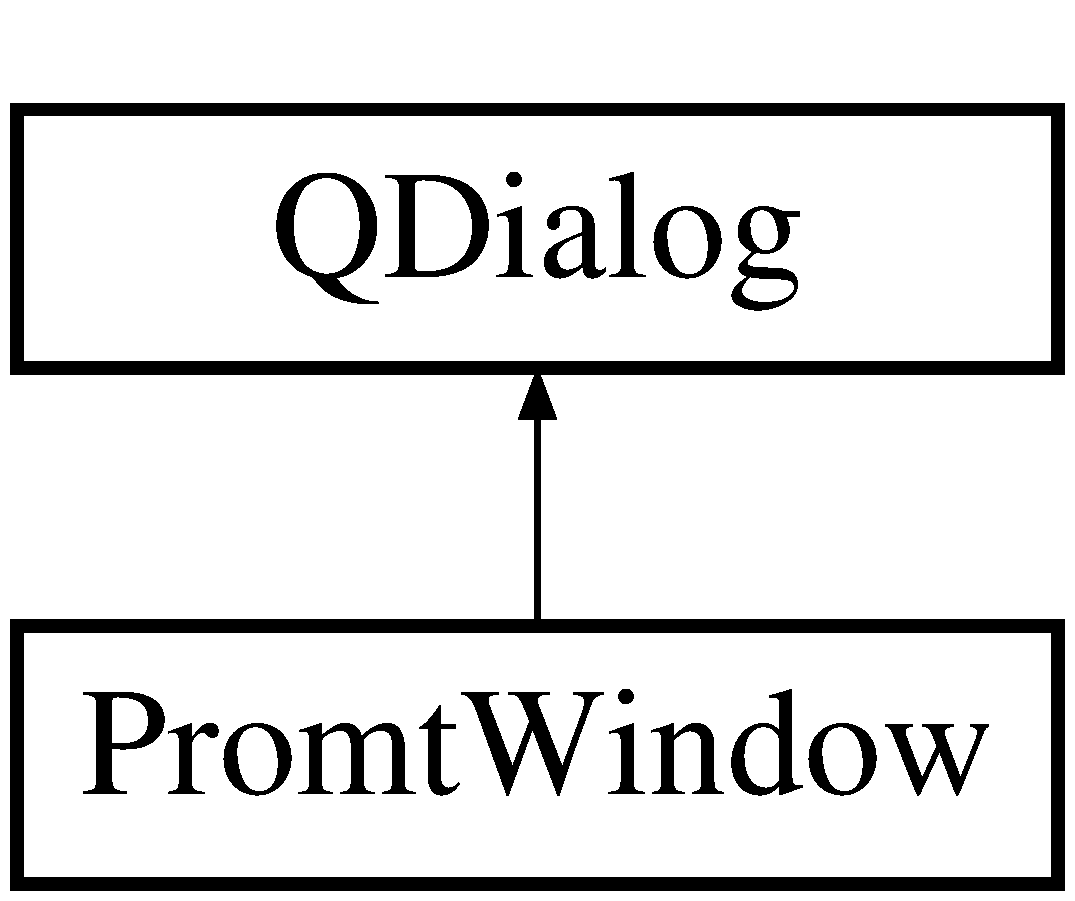
\includegraphics[height=2.000000cm]{classPromtWindow}
\end{center}
\end{figure}
\subsection*{Public Member Functions}
\begin{DoxyCompactItemize}
\item 
\mbox{\hyperlink{classPromtWindow_a6536787a099e6d7348db00b4382244a8}{Promt\+Window}} (Q\+Widget $\ast$parent)
\begin{DoxyCompactList}\small\item\em Constructor for \mbox{\hyperlink{classPromtWindow}{Promt\+Window}}. \end{DoxyCompactList}\item 
void \mbox{\hyperlink{classPromtWindow_a9f2e84ed19a4f520e0e764c31cc39362}{List\+Images}} (Q\+Dir directory)
\begin{DoxyCompactList}\small\item\em List all images in directory. \end{DoxyCompactList}\end{DoxyCompactItemize}


\subsection{Detailed Description}
Implements specific Q\+Dialog. 

\begin{DoxyRemark}{Remarks}
Not used 
\end{DoxyRemark}


Definition at line 34 of file Promt\+Window.\+hpp.



\subsection{Constructor \& Destructor Documentation}
\mbox{\Hypertarget{classPromtWindow_a6536787a099e6d7348db00b4382244a8}\label{classPromtWindow_a6536787a099e6d7348db00b4382244a8}} 
\index{Promt\+Window@{Promt\+Window}!Promt\+Window@{Promt\+Window}}
\index{Promt\+Window@{Promt\+Window}!Promt\+Window@{Promt\+Window}}
\subsubsection{\texorpdfstring{Promt\+Window()}{PromtWindow()}}
{\footnotesize\ttfamily Promt\+Window\+::\+Promt\+Window (\begin{DoxyParamCaption}\item[{Q\+Widget $\ast$}]{parent }\end{DoxyParamCaption})}



Constructor for \mbox{\hyperlink{classPromtWindow}{Promt\+Window}}. 


\begin{DoxyParams}{Parameters}
{\em parent} & The parent Q\+Widget \\
\hline
\end{DoxyParams}


Definition at line 16 of file Promt\+Window.\+cpp.



\subsection{Member Function Documentation}
\mbox{\Hypertarget{classPromtWindow_a9f2e84ed19a4f520e0e764c31cc39362}\label{classPromtWindow_a9f2e84ed19a4f520e0e764c31cc39362}} 
\index{Promt\+Window@{Promt\+Window}!List\+Images@{List\+Images}}
\index{List\+Images@{List\+Images}!Promt\+Window@{Promt\+Window}}
\subsubsection{\texorpdfstring{List\+Images()}{ListImages()}}
{\footnotesize\ttfamily void Promt\+Window\+::\+List\+Images (\begin{DoxyParamCaption}\item[{Q\+Dir}]{directory }\end{DoxyParamCaption})}



List all images in directory. 


\begin{DoxyParams}{Parameters}
{\em directory} & \mbox{\hyperlink{namespacePath}{Path}} to the directory to be listed \\
\hline
\end{DoxyParams}


Definition at line 58 of file Promt\+Window.\+cpp.



The documentation for this class was generated from the following files\+:\begin{DoxyCompactItemize}
\item 
include/\mbox{\hyperlink{PromtWindow_8hpp}{Promt\+Window.\+hpp}}\item 
src/\mbox{\hyperlink{PromtWindow_8cpp}{Promt\+Window.\+cpp}}\end{DoxyCompactItemize}

\hypertarget{structSelectImgToolbar}{}\section{Select\+Img\+Toolbar Struct Reference}
\label{structSelectImgToolbar}\index{Select\+Img\+Toolbar@{Select\+Img\+Toolbar}}


Toolbar used to select image to be cut.  




{\ttfamily \#include $<$G\+U\+I.\+hpp$>$}

\subsection*{Public Attributes}
\begin{DoxyCompactItemize}
\item 
Q\+Tool\+Bar $\ast$ \mbox{\hyperlink{structSelectImgToolbar_a779bc326cf08c9fbcd1ffebb43a664eb}{select\+\_\+img\+\_\+toolbar}}
\item 
Q\+Label $\ast$ \mbox{\hyperlink{structSelectImgToolbar_a3cf6ac92fbe60877873c89939217e1de}{info}}
\item 
Q\+Action $\ast$ \mbox{\hyperlink{structSelectImgToolbar_a82569764f9d7e13b406a668e9e50290a}{continue\+\_\+button}}
\item 
Q\+Action $\ast$ \mbox{\hyperlink{structSelectImgToolbar_a0b17a222dff0441c0f10509315ce9052}{cancel}}
\end{DoxyCompactItemize}


\subsection{Detailed Description}
Toolbar used to select image to be cut. 

Definition at line 155 of file G\+U\+I.\+hpp.



\subsection{Member Data Documentation}
\mbox{\Hypertarget{structSelectImgToolbar_a0b17a222dff0441c0f10509315ce9052}\label{structSelectImgToolbar_a0b17a222dff0441c0f10509315ce9052}} 
\index{Select\+Img\+Toolbar@{Select\+Img\+Toolbar}!cancel@{cancel}}
\index{cancel@{cancel}!Select\+Img\+Toolbar@{Select\+Img\+Toolbar}}
\subsubsection{\texorpdfstring{cancel}{cancel}}
{\footnotesize\ttfamily Q\+Action$\ast$ Select\+Img\+Toolbar\+::cancel}

Pointer to a Q\+Action which connects to Cancel\+From\+Select 

Definition at line 160 of file G\+U\+I.\+hpp.

\mbox{\Hypertarget{structSelectImgToolbar_a82569764f9d7e13b406a668e9e50290a}\label{structSelectImgToolbar_a82569764f9d7e13b406a668e9e50290a}} 
\index{Select\+Img\+Toolbar@{Select\+Img\+Toolbar}!continue\+\_\+button@{continue\+\_\+button}}
\index{continue\+\_\+button@{continue\+\_\+button}!Select\+Img\+Toolbar@{Select\+Img\+Toolbar}}
\subsubsection{\texorpdfstring{continue\+\_\+button}{continue\_button}}
{\footnotesize\ttfamily Q\+Action$\ast$ Select\+Img\+Toolbar\+::continue\+\_\+button}

Pointer to a Q\+Action which connects to Continue\+From\+Select 

Definition at line 159 of file G\+U\+I.\+hpp.

\mbox{\Hypertarget{structSelectImgToolbar_a3cf6ac92fbe60877873c89939217e1de}\label{structSelectImgToolbar_a3cf6ac92fbe60877873c89939217e1de}} 
\index{Select\+Img\+Toolbar@{Select\+Img\+Toolbar}!info@{info}}
\index{info@{info}!Select\+Img\+Toolbar@{Select\+Img\+Toolbar}}
\subsubsection{\texorpdfstring{info}{info}}
{\footnotesize\ttfamily Q\+Label$\ast$ Select\+Img\+Toolbar\+::info}

Label used to inform user 

Definition at line 158 of file G\+U\+I.\+hpp.

\mbox{\Hypertarget{structSelectImgToolbar_a779bc326cf08c9fbcd1ffebb43a664eb}\label{structSelectImgToolbar_a779bc326cf08c9fbcd1ffebb43a664eb}} 
\index{Select\+Img\+Toolbar@{Select\+Img\+Toolbar}!select\+\_\+img\+\_\+toolbar@{select\+\_\+img\+\_\+toolbar}}
\index{select\+\_\+img\+\_\+toolbar@{select\+\_\+img\+\_\+toolbar}!Select\+Img\+Toolbar@{Select\+Img\+Toolbar}}
\subsubsection{\texorpdfstring{select\+\_\+img\+\_\+toolbar}{select\_img\_toolbar}}
{\footnotesize\ttfamily Q\+Tool\+Bar$\ast$ Select\+Img\+Toolbar\+::select\+\_\+img\+\_\+toolbar}

Pointer to the Q\+Tool\+Bar 

Definition at line 157 of file G\+U\+I.\+hpp.



The documentation for this struct was generated from the following file\+:\begin{DoxyCompactItemize}
\item 
include/\mbox{\hyperlink{GUI_8hpp}{G\+U\+I.\+hpp}}\end{DoxyCompactItemize}

\chapter{File Documentation}
\hypertarget{gui_8hpp}{}\section{include/gui.hpp File Reference}
\label{gui_8hpp}\index{include/gui.\+hpp@{include/gui.\+hpp}}


Header for \mbox{\hyperlink{classGUI}{G\+UI}} class.  


{\ttfamily \#include $<$Q\+Main\+Window$>$}\newline
{\ttfamily \#include $<$Q\+Widget$>$}\newline
{\ttfamily \#include $<$Q\+Application$>$}\newline
{\ttfamily \#include $<$Q\+Menu$>$}\newline
{\ttfamily \#include $<$Q\+Menu\+Bar$>$}\newline
{\ttfamily \#include $<$Q\+Tool\+Bar$>$}\newline
{\ttfamily \#include $<$Q\+Icon$>$}\newline
{\ttfamily \#include $<$Q\+Mouse\+Event$>$}\newline
{\ttfamily \#include $<$Q\+Debug$>$}\newline
{\ttfamily \#include $<$Q\+Graphics\+Scene$>$}\newline
{\ttfamily \#include $<$Q\+Graphics\+View$>$}\newline
{\ttfamily \#include $<$Q\+Graphics\+Item$>$}\newline
{\ttfamily \#include $<$Q\+Box\+Layout$>$}\newline
{\ttfamily \#include $<$Q\+Point$>$}\newline
{\ttfamily \#include $<$Q\+Push\+Button$>$}\newline
{\ttfamily \#include $<$Q\+Image$>$}\newline
{\ttfamily \#include $<$Q\+Painter$>$}\newline
{\ttfamily \#include $<$Q\+File\+Dialog$>$}\newline
{\ttfamily \#include $<$Q\+Message\+Box$>$}\newline
{\ttfamily \#include $<$Q\+String$>$}\newline
{\ttfamily \#include $<$Q\+Dir$>$}\newline
{\ttfamily \#include $<$Q\+String\+List$>$}\newline
{\ttfamily \#include $<$Q\+Tool\+Button$>$}\newline
{\ttfamily \#include $<$Q\+Label$>$}\newline
{\ttfamily \#include $<$Q\+Combo\+Box$>$}\newline
{\ttfamily \#include \char`\"{}owngraphicsscene.\+hpp\char`\"{}}\newline
{\ttfamily \#include \char`\"{}mainwidget.\+hpp\char`\"{}}\newline
{\ttfamily \#include \char`\"{}combobox\+\_\+action.\+hpp\char`\"{}}\newline
\subsection*{Classes}
\begin{DoxyCompactItemize}
\item 
struct \mbox{\hyperlink{structPolygonToolbar}{Polygon\+Toolbar}}
\begin{DoxyCompactList}\small\item\em Toolbar used in image polygon cut. \end{DoxyCompactList}\item 
struct \mbox{\hyperlink{structModeToolbar}{Mode\+Toolbar}}
\begin{DoxyCompactList}\small\item\em Toolbar for changing image cut mode. \end{DoxyCompactList}\item 
struct \mbox{\hyperlink{structSelectImgToolbar}{Select\+Img\+Toolbar}}
\begin{DoxyCompactList}\small\item\em Toolbar used to select image to be cut. \end{DoxyCompactList}\item 
class \mbox{\hyperlink{classGUI}{G\+UI}}
\begin{DoxyCompactList}\small\item\em Graphical user interface. \end{DoxyCompactList}\end{DoxyCompactItemize}
\subsection*{Macros}
\begin{DoxyCompactItemize}
\item 
\mbox{\Hypertarget{gui_8hpp_a478a74bc43cef5db4fb68806bb3a3045}\label{gui_8hpp_a478a74bc43cef5db4fb68806bb3a3045}} 
\#define \mbox{\hyperlink{gui_8hpp_a478a74bc43cef5db4fb68806bb3a3045}{exit\+\_\+img}}~\char`\"{}img\+\_\+src/exit.\+png\char`\"{}
\begin{DoxyCompactList}\small\item\em Exit image macro. \end{DoxyCompactList}\item 
\mbox{\Hypertarget{gui_8hpp_a90a466ca632ac85ebbd176bba62a8fed}\label{gui_8hpp_a90a466ca632ac85ebbd176bba62a8fed}} 
\#define \mbox{\hyperlink{gui_8hpp_a90a466ca632ac85ebbd176bba62a8fed}{open\+\_\+img}}~\char`\"{}img\+\_\+src/open.\+png\char`\"{}
\begin{DoxyCompactList}\small\item\em Open image macro. \end{DoxyCompactList}\item 
\mbox{\Hypertarget{gui_8hpp_ae14474955e229d006688f31321aeef30}\label{gui_8hpp_ae14474955e229d006688f31321aeef30}} 
\#define \mbox{\hyperlink{gui_8hpp_ae14474955e229d006688f31321aeef30}{save\+\_\+img}}~\char`\"{}img\+\_\+src/save.\+png\char`\"{}
\begin{DoxyCompactList}\small\item\em Save image macro. \end{DoxyCompactList}\item 
\mbox{\Hypertarget{gui_8hpp_a7f04d211e7913a5261475b88fd66b777}\label{gui_8hpp_a7f04d211e7913a5261475b88fd66b777}} 
\#define \mbox{\hyperlink{gui_8hpp_a7f04d211e7913a5261475b88fd66b777}{draw\+\_\+line\+\_\+img}}~\char`\"{}img\+\_\+src/draw\+\_\+line.\+png\char`\"{}
\begin{DoxyCompactList}\small\item\em Draw line image macro. \end{DoxyCompactList}\item 
\mbox{\Hypertarget{gui_8hpp_abac07b84eaf5bfe1b574356adf52ce42}\label{gui_8hpp_abac07b84eaf5bfe1b574356adf52ce42}} 
\#define \mbox{\hyperlink{gui_8hpp_abac07b84eaf5bfe1b574356adf52ce42}{delete\+\_\+line\+\_\+img}}~\char`\"{}img\+\_\+src/delete\+\_\+line.\+png\char`\"{}
\begin{DoxyCompactList}\small\item\em Delete line image macro. \end{DoxyCompactList}\item 
\mbox{\Hypertarget{gui_8hpp_a3e0477dc697ad2153357f9c02f19431b}\label{gui_8hpp_a3e0477dc697ad2153357f9c02f19431b}} 
\#define \mbox{\hyperlink{gui_8hpp_a3e0477dc697ad2153357f9c02f19431b}{clear\+\_\+points\+\_\+img}}~\char`\"{}img\+\_\+src/clear\+\_\+points.\+png\char`\"{}
\begin{DoxyCompactList}\small\item\em Clear points image macro. \end{DoxyCompactList}\item 
\mbox{\Hypertarget{gui_8hpp_a63e6f9ee3d2bc3cb839909281ac5d807}\label{gui_8hpp_a63e6f9ee3d2bc3cb839909281ac5d807}} 
\#define \mbox{\hyperlink{gui_8hpp_a63e6f9ee3d2bc3cb839909281ac5d807}{clear\+\_\+all\+\_\+img}}~\char`\"{}img\+\_\+src/clear\+\_\+all.\+png\char`\"{}
\begin{DoxyCompactList}\small\item\em Clear all image macro. \end{DoxyCompactList}\item 
\mbox{\Hypertarget{gui_8hpp_a3e5269f105011bf3ef8a4efc2cf3ccbf}\label{gui_8hpp_a3e5269f105011bf3ef8a4efc2cf3ccbf}} 
\#define \mbox{\hyperlink{gui_8hpp_a3e5269f105011bf3ef8a4efc2cf3ccbf}{image\+\_\+sketch\+\_\+img}}~\char`\"{}img\+\_\+src/image\+\_\+sketch.\+png\char`\"{}
\begin{DoxyCompactList}\small\item\em Image sketch macro. \end{DoxyCompactList}\item 
\mbox{\Hypertarget{gui_8hpp_ae0967b0632586ee3481fbdacff2858e3}\label{gui_8hpp_ae0967b0632586ee3481fbdacff2858e3}} 
\#define \mbox{\hyperlink{gui_8hpp_ae0967b0632586ee3481fbdacff2858e3}{image\+\_\+delete\+\_\+img}}~\char`\"{}img\+\_\+src/image\+\_\+delete.\+png\char`\"{}
\begin{DoxyCompactList}\small\item\em Image delete image macro. \end{DoxyCompactList}\item 
\mbox{\Hypertarget{gui_8hpp_aa390e86a16a72f2efc028e0434c4bd15}\label{gui_8hpp_aa390e86a16a72f2efc028e0434c4bd15}} 
\#define \mbox{\hyperlink{gui_8hpp_aa390e86a16a72f2efc028e0434c4bd15}{image\+\_\+cut\+\_\+img}}~\char`\"{}img\+\_\+src/image\+\_\+cut.\+png\char`\"{}
\begin{DoxyCompactList}\small\item\em Image cut image macro. \end{DoxyCompactList}\item 
\mbox{\Hypertarget{gui_8hpp_ac646c2d9dc5338391faa385199532ead}\label{gui_8hpp_ac646c2d9dc5338391faa385199532ead}} 
\#define \mbox{\hyperlink{gui_8hpp_ac646c2d9dc5338391faa385199532ead}{continue\+\_\+img}}~\char`\"{}img\+\_\+src/continue.\+png\char`\"{}
\begin{DoxyCompactList}\small\item\em Continue image macro. \end{DoxyCompactList}\item 
\mbox{\Hypertarget{gui_8hpp_a9f228b0281863ba576bea09d2fb86f98}\label{gui_8hpp_a9f228b0281863ba576bea09d2fb86f98}} 
\#define \mbox{\hyperlink{gui_8hpp_a9f228b0281863ba576bea09d2fb86f98}{cancel\+\_\+img}}~\char`\"{}img\+\_\+src/cancel.\+png\char`\"{}
\begin{DoxyCompactList}\small\item\em Cancel image macro. \end{DoxyCompactList}\item 
\mbox{\Hypertarget{gui_8hpp_ab0bdf7d170572d6e0905dfb4dbc9f883}\label{gui_8hpp_ab0bdf7d170572d6e0905dfb4dbc9f883}} 
\#define \mbox{\hyperlink{gui_8hpp_ab0bdf7d170572d6e0905dfb4dbc9f883}{finish\+\_\+img}}~\char`\"{}img\+\_\+src/finish.\+png\char`\"{}
\begin{DoxyCompactList}\small\item\em Finish image macro. \end{DoxyCompactList}\item 
\mbox{\Hypertarget{gui_8hpp_a19fb1ba48d0a34f41020472dd625cf95}\label{gui_8hpp_a19fb1ba48d0a34f41020472dd625cf95}} 
\#define \mbox{\hyperlink{gui_8hpp_a19fb1ba48d0a34f41020472dd625cf95}{remove\+\_\+point\+\_\+img}}~\char`\"{}img\+\_\+src/remove\+\_\+point.\+png\char`\"{}
\begin{DoxyCompactList}\small\item\em Remove point image macro. \end{DoxyCompactList}\item 
\mbox{\Hypertarget{gui_8hpp_a2f3a39a019b38e118882c2a5e79d90a3}\label{gui_8hpp_a2f3a39a019b38e118882c2a5e79d90a3}} 
\#define \mbox{\hyperlink{gui_8hpp_a2f3a39a019b38e118882c2a5e79d90a3}{bezier\+\_\+pic\+\_\+img}}~\char`\"{}img\+\_\+src/bezier\+\_\+pic.\+png\char`\"{}
\begin{DoxyCompactList}\small\item\em \mbox{\hyperlink{classBezier}{Bezier}} pic image macro. \end{DoxyCompactList}\end{DoxyCompactItemize}


\subsection{Detailed Description}
Header for \mbox{\hyperlink{classGUI}{G\+UI}} class. 

\begin{DoxyAuthor}{Author}
Lauri Westerholm 
\end{DoxyAuthor}

%--- End generated contents ---

% Index
\backmatter
\newpage
\phantomsection
\clearemptydoublepage
\addcontentsline{toc}{chapter}{Index}
\printindex

\end{document}
